\section{Overview}
\label{sec:overview}%

The architectural design of the S\&C system is based on a modular and scalable 4-tier architecture. This structure ensures a clear separation of responsibilities, improves maintainability, and supports efficient interactions between components. The application is designed to provide a seamless platform for students, companies, and universities to manage and interact with internships through an integrated system.

\begin{figure}[H]
    \centering
    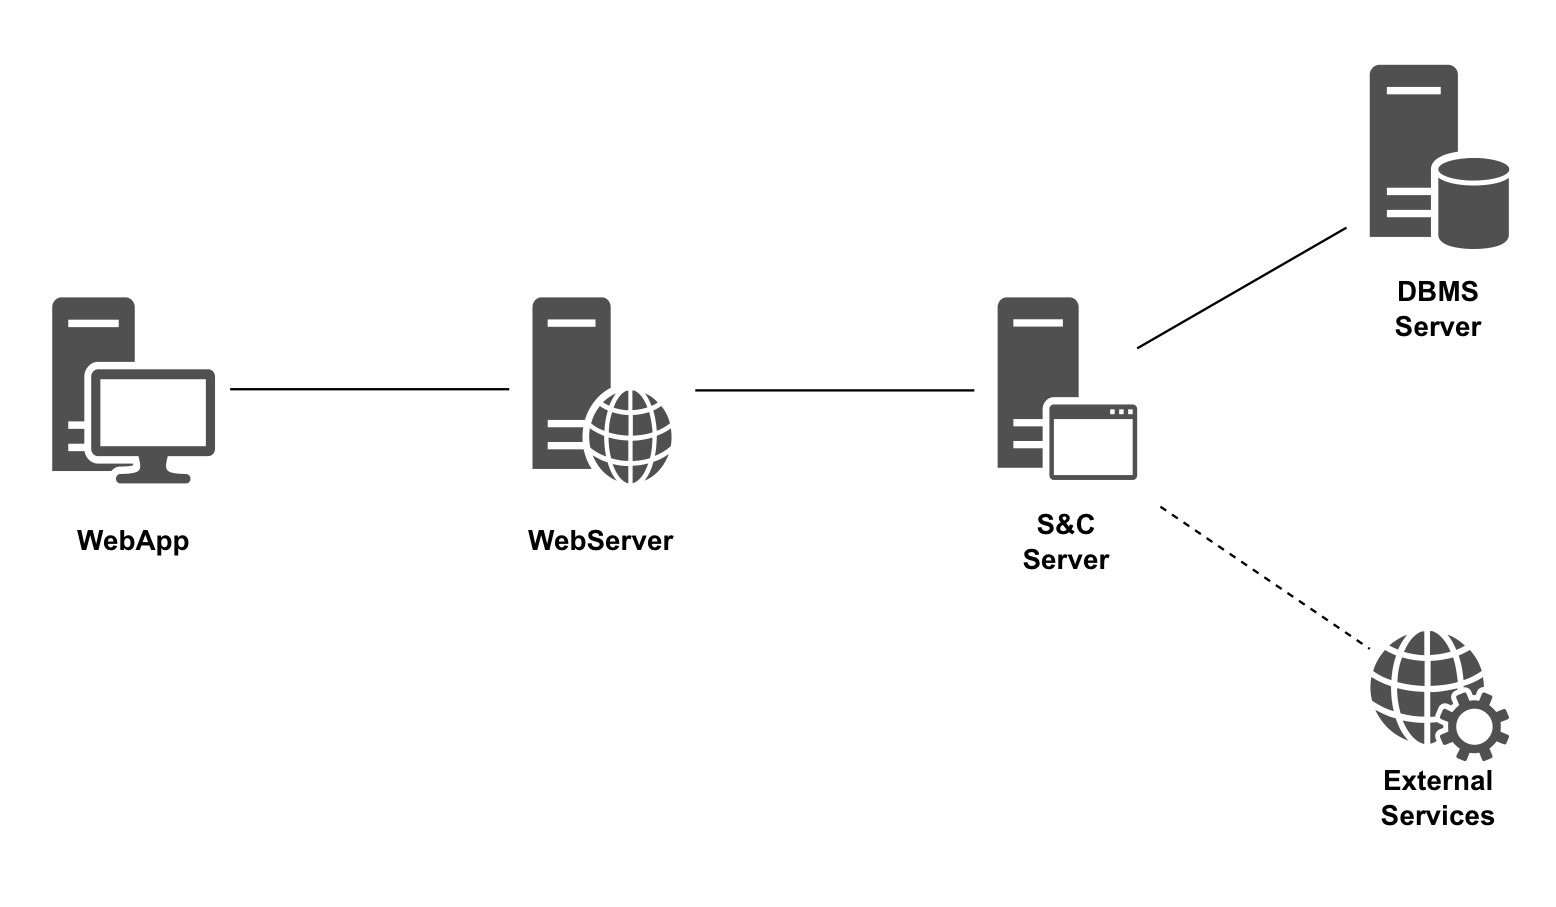
\includegraphics[width=\linewidth]{DD/Images/overview.jpg}
    \caption{Four tier architecture.}
    \label{fig:overview}
\end{figure}

\newpage

The four tiers of the architecture are:

\begin{itemize}
    \item
        \textbf{Web Application (Presentation Layer):} Acts as the external access point for users, providing an intuitive and responsive user interface.
    \item 
        \textbf{Web Server:} Handles communication between the web application and the application server, managing incoming requests and responses.
    \item 
        \textbf{Application Server (Business Logic Layer):} Hosts the core business logic of the system, processing data and coordinating operations.
    \item 
        \textbf{Database (Data Layer):} Stores all persistent data, ensuring secure and efficient retrieval and updates.
\end{itemize}

This 4-tier architecture ensures that the system can handle complex operations while maintaining high performance and scalability.

\newpage

\section{Component View}
\label{sec:component_view}

The component diagram below illustrates the primary components of the system and their interactions across the four tiers. External Systems, such as AI Tools, Data Analytics Service and eMail Provider, are presented as black-boxes that expose only the interfaces used by the system. 

\begin{figure}[htbp]
    \centering
    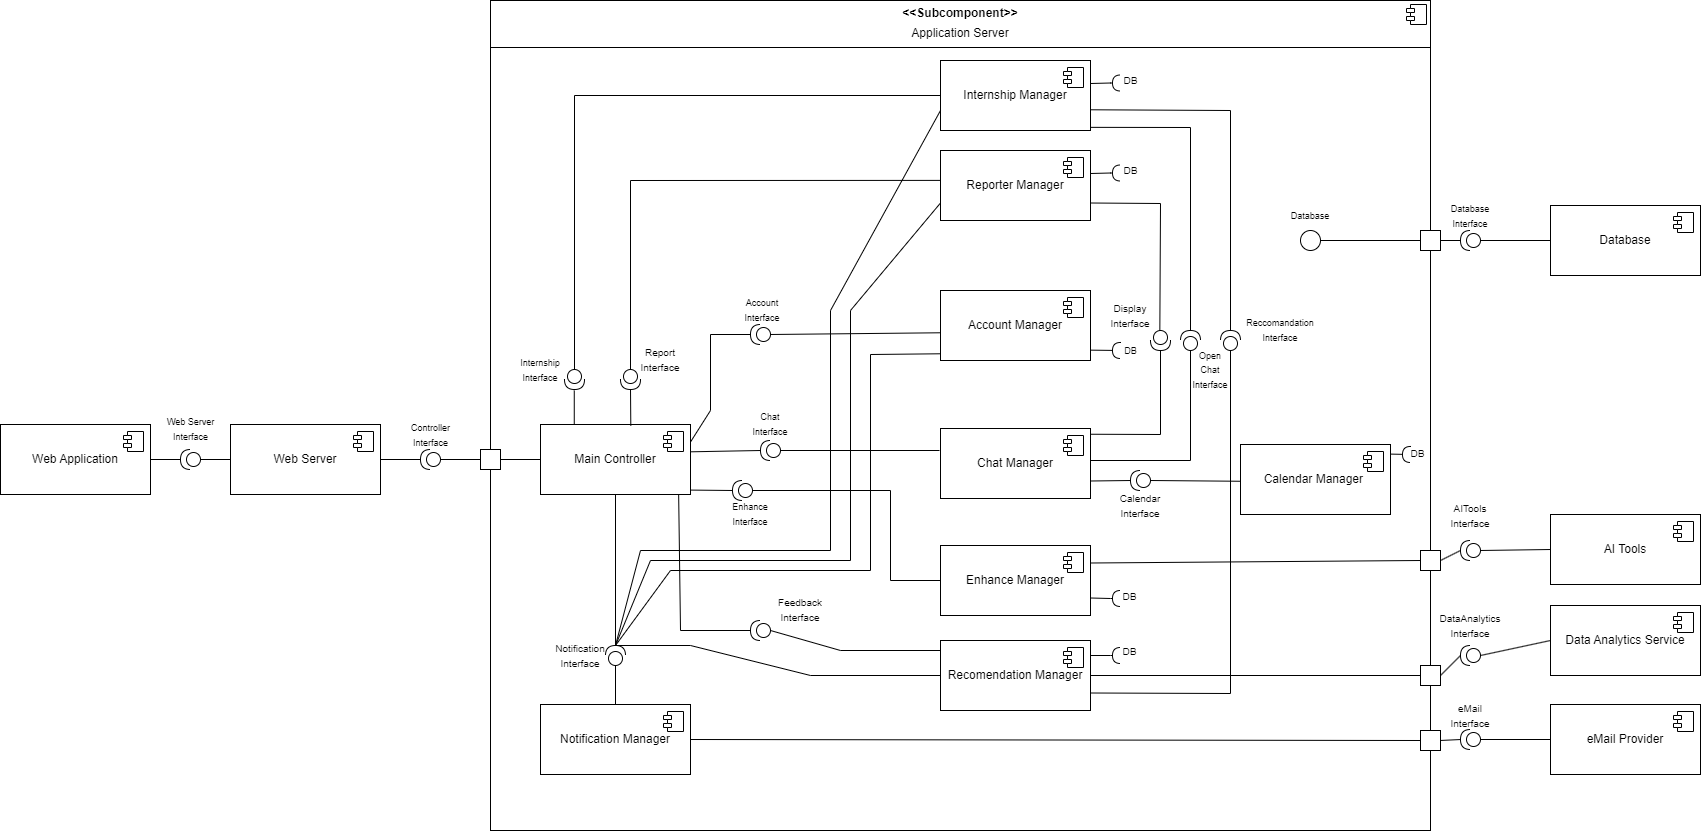
\includegraphics[width=\linewidth]{DD/Images/Comp&Sub/LLD.png}
    \caption{Component diagram.}
    \label{fig:component_diagram}
\end{figure}


\subsection{Presentation Layer}
\label{subsec:presentation_layer}%

The presentation layer serves as the external interface for users (students, companies, and universities). It represents the front-end of the system, including only the ability to perform very basic checks such as the recognitions of empty or incomplete forms, all other parts of the logic are entirely handled by the application server.

As shown before, this layer contains the Web Application that provides a responsive interface for accessing the system through different web browsers.


\subsection{Web Server}
\label{subsec:web_server}%

Acts as the intermediary between the web application and the application server, it indeed processes HTTP/HTTPS requests from the web application, forwards requests to the application server and sends back responses. It ensures secure and reliable communication between the user-facing frontend and backend services.


\subsection{Application Server (Business Logic Layer):}
\label{subsec:application_server}%

The application server hosts the core functionalities and business rules of the system, including all the logic, and coordinates the information between the presentation layer and the data layer.

As shown before, this layer contain several components:
\subsubsection{Main Controller}
The Main Controller serves as the central node for communication and coordination within the Application Server. It ensures the proper routing of data and requests between the Web Server and the various backend managers, acting as the primary mediator between the Web Application and the backend services.
It simplifies system architecture by managing the complexity of data flow and interactions between components. This design enhances system efficiency and reduces errors, providing a streamlined mechanism for backend operations.

\subsubsection{Account Manager}
         Manages user authentication, account information, including updates and role assignments. It communicates with the Database in order to verify, access, store and delete account information. Indeed, this component is responsible for account creation and for the authentication process.
    
    \begin{figure}[H]
    \centering
    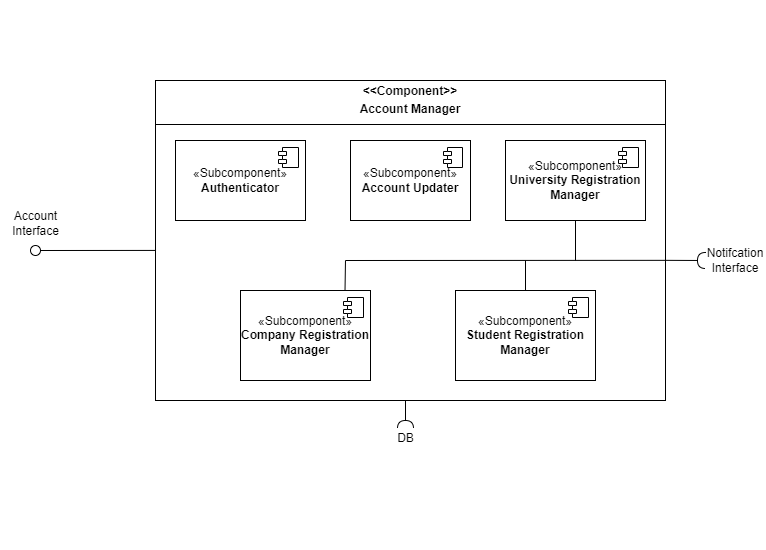
\includegraphics[width=0.7\linewidth]{DD/Images/Comp&Sub/Account Manager.png}
    \caption{Subcomponent diagram Account Manager}
    \label{fig:account_manager}
    \end{figure}

   It consists of the following subcomponents:
   \begin{itemize}
    \item  \textbf{Authenticator}: this subcomponent handles the authentications of the users by checking the credentials.
    \item  \textbf{AccountUpdater}: it is responsible for updating account data and deleting the account.
    \item  \textbf{University Registration Manager}: it manages the registration and the assignment of the role to new universities.
    \item  \textbf{Company Registration Manager}: it manages the registration and the assignment of the role to new companies.
    \item  \textbf{Student Registration Manager}: it manages the registration and the assignment of the role to new students.
    \end{itemize}

\newpage

\subsubsection{Notification Manager}Processes and sends notifications, in real time as required, to all users. Sends an in-app notification and an email using the interface provided by the email provider.Additionally, it utilizes its own interface to listen for all possible events that may occur.
   
\begin{figure}[H]
    \centering
    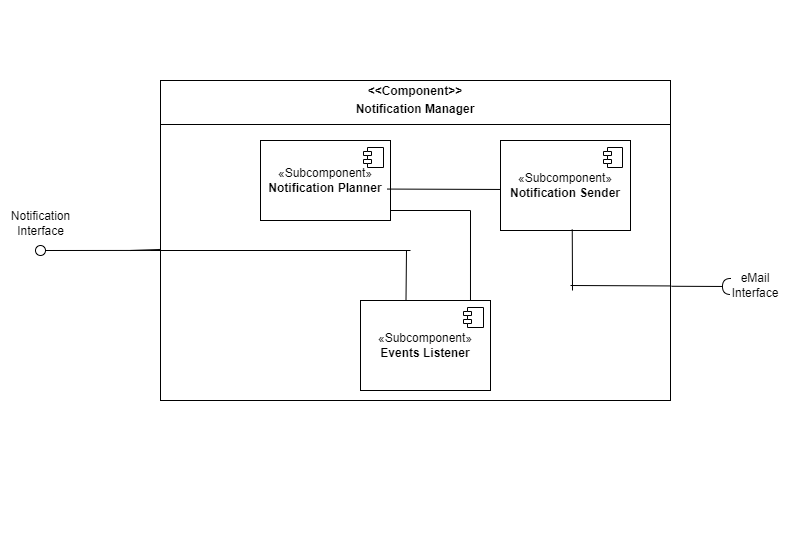
\includegraphics[width=\linewidth]{DD/Images/Comp&Sub/NotificationManager.png}
    \caption{Subcomponent diagram Notification Manager}
    \label{fig:notification_manager}
\end{figure}
    
It consists of the following subcomponents:
\begin{itemize}
    \item  \textbf{Notification Planner}: It manages the registration of events that trigger the delivery of notifications.
    \item  \textbf{Notification Sender}:It handles the actual delivery of notifications to the Web Application.
    \item  \textbf{Events Listener}: It is responsible for detecting the occurrence of events that trigger the notification delivery.
    \end{itemize}
 \clearpage % Forza l'inizio di una nuova pagina
\subsubsection{Internship Manager} Manages internship listings, including modifications and status updates, while also overseeing the collection of all applications submitted by students.  It communicates with the Database in order to verify, access, store and delete internship information.
    \begin{figure}[H]
    \centering
    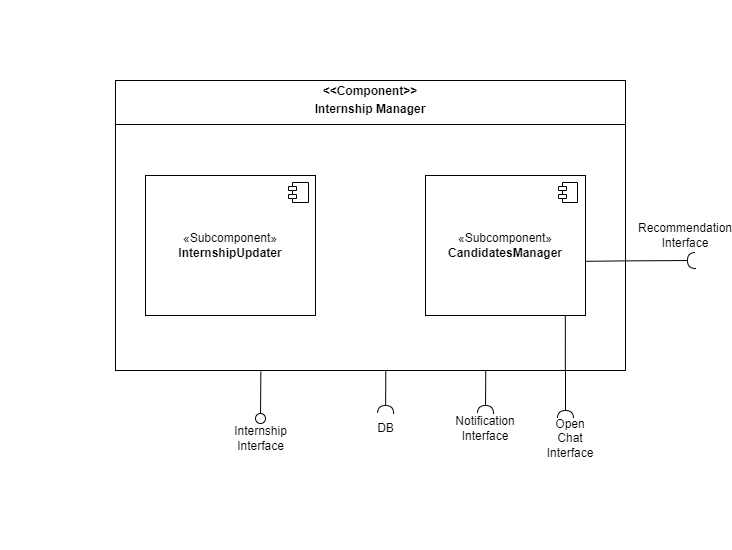
\includegraphics[width=\linewidth]{DD/Images/Comp&Sub/InternshipManager.png}
    \caption{Subcomponent diagram Internship Manager.}
    \label{fig:internship_manager}
    \end{figure}
    
It consists of the following subcomponents:
\begin{itemize}
    \item  \textbf{Internship Updater}: it manages every kind of update made to the internships.
    \item  \textbf{Candidate Manager}: it collects every candidate that made application for each internship
    \end{itemize}

\clearpage % Forza l'inizio di una nuova pagina
\subsubsection{Chat Manager} Facilitates real-time communication among students, companies, and universities by managing messages, interviews, and offers. Additionally, it interacts with the database to verify, access, store, and delete messages along with their associated timestamps. Finally, it is responsible for handling the submission of complaints and, if necessary, closing a chat.
\begin{figure}[H]
    \centering
    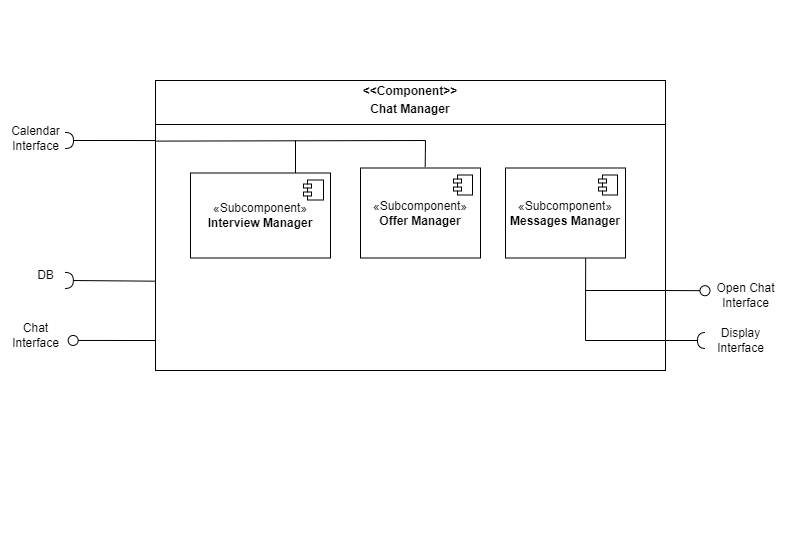
\includegraphics[width=0.8\linewidth]{DD/Images/Comp&Sub/ChatManager.png}
    \caption{Subcomponent diagram Chat Manager.}
    \label{fig:chat_manager}
    \end{figure}
    
It consists of the following subcomponents:
\begin{itemize}
    \item  \textbf{Interview Manager}: It is responsible for managing interview proposals made by companies and adding the event to the calendar.
    \item  \textbf{Offer Manager}: It is responsible for managing contract proposals made by companies and, in the case of a positive outcome, adding the start and end dates of the internship to the calendar.
    \item  \textbf{Messages Manager}: It is responsible for facilitating communication between the two parties, ensuring a real-time chat experience with zero delays and no loss of information.
    It also takes part in the potential process of terminating an internship by offering the interface for closing the chat.
    \end{itemize}

\subsubsection{Calendar Manager} Manages events and schedules for internships and deadlines, while providing an interface for other components to add potential events to the calendar.

 
\subsubsection{Enhance Manager} It aims to provide services integrated with AI Tools to offer suggestions regarding CVs and internship postings.
 \begin{figure}[H]
    \centering
    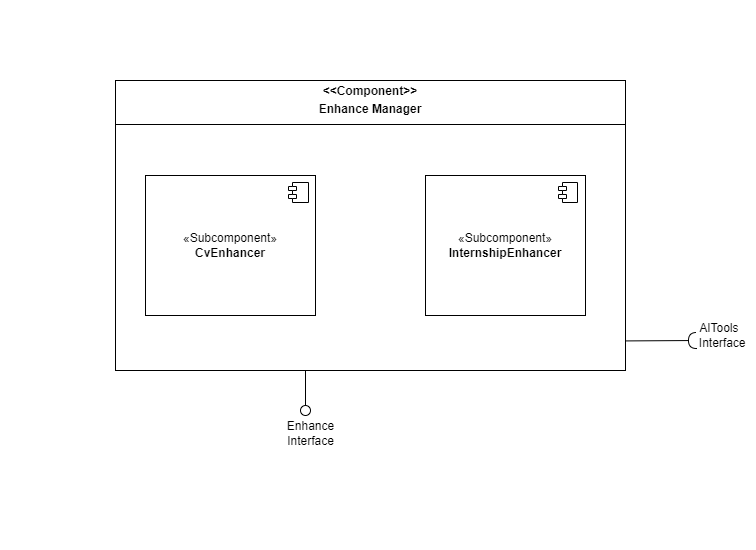
\includegraphics[width=\linewidth]{DD/Images/Comp&Sub/EnhanceManager.png}
    \caption{Subcomponent diagram Enhance Manager.}
    \label{fig:enhance_manager}
    \end{figure}

It consists of the following subcomponents:
\begin{itemize}
    \item  \textbf{Cv Enhancer}: It assists students in enhancing their CVs by analyzing them and providing improvement suggestions through AI tools.
    \item  \textbf{Internship Enhancer}: It assists companies in improving their postings by analyzing them and providing suggestions for enhancements through AI tools.
    \end{itemize}
    

\subsubsection{Recommendation Manager} It aims to provide personalized suggestions by leveraging external data analytics services and all data stored in the database, in addition to deliver real-time suggestions, it utilizes the notification interface. Finally it also handles feedback's submission.
 \begin{figure}[H]
    \centering
    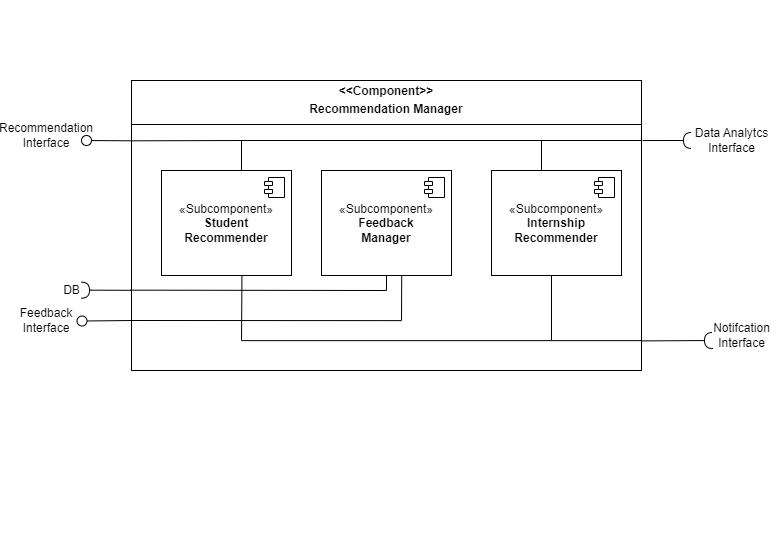
\includegraphics[width=\linewidth]{DD/Images/Comp&Sub/ReccomandationManager.png}
    \caption{Subcomponent diagram Recomendation Manager.}
    \label{fig:reccomendation_manager}
    \end{figure}

    It consists of the following subcomponents:
\begin{itemize}
    \item  \textbf{Student Recommender}: It is responsible for managing the recommendations generated for students.
    \item  \textbf{Internship Recommender}: It is responsible for managing the recommendations generated for companies.
    \item  \textbf{Feedback Manager}:It is responsible for collecting feedback and saving it in the database, ensuring it can be utilized for generating recommendations.
    \end{itemize}
    
 \clearpage % Forza l'inizio di una nuova pagina
\subsubsection{Reporter Manager} It is responsible for providing interfaces to the chat for uploading information or submitting complaints during an internship. It is also responsible for managing and storing them, and, if deemed necessary by the university, requesting the closure of the chat through the interface provided by the chat manager.
\begin{figure}[H]
    \centering
    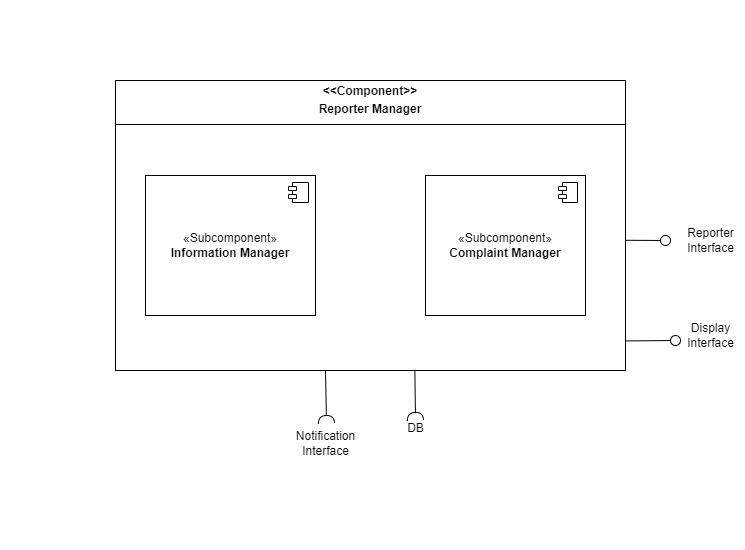
\includegraphics[width=\linewidth]{DD/Images/Comp&Sub/ComplaintManager.png}
    \caption{Subcomponent diagram Reporter Manager.}
    \label{fig:report_manager}
    \end{figure}
    
It consists of the following subcomponents:
\begin{itemize}
    \item  \textbf{Information Manager}: it handles every information added through the chat.
    \item  \textbf{Complaint Manager}: It stores and handles all complaints submitted via the chat and, if necessary, is responsible for closing the chat through the corresponding interface.
    \end{itemize}

\clearpage % Forza l'inizio di una nuova pagina

\subsection{Database (Data Layer)}
\label{subsec:data_layer}%

The Database serves as centralized storage for all application data, directly connected to the Application Server for all read and write operations. It ensures data consistency and supports efficient querying through a well-structured relational model, optimized with indexing and normalization. 

Designed with strict access controls, it guarantees secure interactions, with only authorized components managing data. The Database supports seamless integration with the Application Server via defined interfaces, ensuring a clear separation of concerns. Backup and recovery mechanisms further enhance reliability, making it a robust and efficient foundation for the system's data management needs.

\subsection{External Systems}
\label{subsec:external_systems}%

These external system communicates with the \textit{Application Server} via APIs.

\begin{itemize}
    \item
        \textbf{AI Tools:} Enhance user CVs and internship descriptions with intelligent processing.
    \item
        \textbf{Data Analytics Services:} Provide insights and recommendations for internships based on user preferences and behavior.
        \item 
        \textbf{Email Provider:} Sends notification emails to users through the Notification Manager.
\end{itemize}

\newpage 

\section{Deployment View}
\label{sec:deployment_view}

The deployment view represents the architecture that separates the system into the Presentation Tier, Application Tier (divided in Web Server and Application Server) and Data Tier, ensuring modularity, scalability, and maintainability.

\begin{figure}[H]
    \centering
    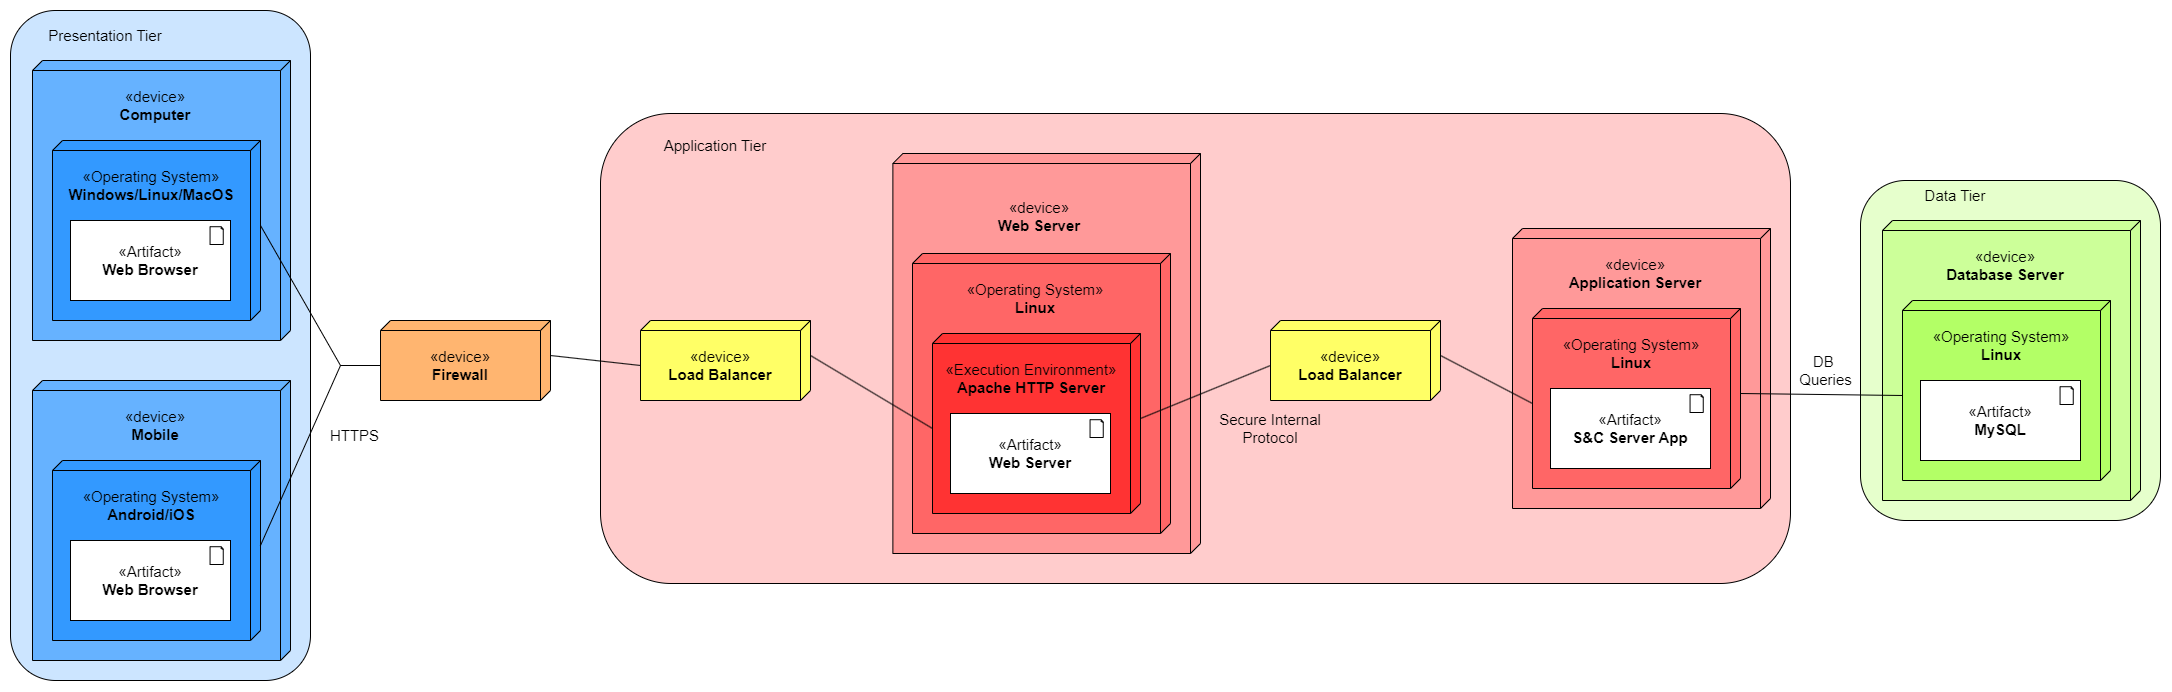
\includegraphics[width=\linewidth]{DD/Images/deploymentView.png}
    \caption{Deployment view.}
    \label{fig:deployment_view}
\end{figure}

\begin{itemize}
    \item 
        \textbf{Presentation Tier:} Includes computers (Windows/Linux/macOS) and mobile devices (Android/iOS). These devices host web browsers that serve as the interface for users (students, companies, and universities). The communication between the devices and the system passes through a Firewall to ensure secure external connections. All communication is secured via HTTPS.
    \item 
        \textbf{Application Tier:} The Firewall acts as the first layer of defense for incoming connections. Load Balancers are used at both the Web Server and Application Server levels to distribute requests evenly, prevent overload, and ensure high availability.
        \begin{itemize}
            \item 
                \textbf{Web Server:}
                    Hosted on a Linux environment, the Web Server uses an Apache HTTP Server as its execution environment. The Web Server handles incoming HTTP/HTTPS requests from the Presentation Tier and forwards them to the Application Server.
            \item 
                \textbf{Application Server:}
                    Also hosted on a Linux environment, the Application Server contains the S\&C Server App, which implements the business logic of the system. Communicates with both the Web Server and the Database Server.
        \end{itemize}
    \item 
        \textbf{Data Tier:} It's the Database Server, a centralized storage system running on Linux. The MySQL artifact manages all application data, ensuring consistency and supporting efficient querying. Directly connected to the Application Server for all read/write operations, enabling real-time updates and reliability.
\end{itemize}

\subsection{Key Architectural Choices}

\begin{itemize}
    \item The architecture follows a clear separation of concerns by isolating the user interface, application logic, and data management into distinct tiers. This modular design enhances scalability and simplifies system maintenance.
    
    \item The database employs a centralized storage strategy, serving as a single source of truth to eliminate data duplication and ensure consistency across the system.
    
    \item Security is prioritized through the use of HTTPS for all external communications and secure internal protocols between system components, safeguarding data and preventing unauthorized access.
    
    \item Load balancers are strategically integrated to manage increased traffic, distribute requests evenly, and maintain high system availability under varying loads.
\end{itemize}

\newpage

\section{Component Interfaces}
\label{sec:component_interfaces}

\subsection{Account Interface}
The \textbf{Account Interface}, offered by the Account Manager, helps the Main Controller to manage user account operationns. Its key methods and corresponding functionalities are as follows:
\begin{itemize}
    \item \texttt{createAccount()}: It allows the callback of a new form to be filled in for account creation via the \textit{Account Manager}.
    \item \texttt{SignUp(userdata UserData)}: It allows managing the user registration process through the \textit{Account Manager}.
    \item \texttt{selectRole(string Role)}: It allows role selection during registration or login by interacting with the \textit{Authenticator}.
    \item \texttt{login(String email, String password)}: It allows authenticating the user through the \textit{Authenticator}.
    \item \texttt{openProfile(profile Profile)}: It allows opening the personal profile page using the \textit{AccountUpdater}.
    \item \texttt{search(string CompanyName)}: It allows searching for company profiles using the \textit{AccountUpdater}.
    \item \texttt{ClickOnCompany(profile Company)}: It allows accessing a company’s profile during a search via the \textit{AccountUpdater}.
    \item \texttt{clickOnProfile(profile Profile)}: It allows viewing another user’s profile using the \textit{AccountUpdater}.
    \item \texttt{clickOnNotification()}: It allows managing notification interactions via the \textit{AccountUpdater}.
\end{itemize}

\subsection{Internship Interface}
The \textbf{Internship Interface}, offered by Internship Manager, helps the Main Controller in managing internships and candidates. Its methods include:
\begin{itemize}
    \item \texttt{postInternship()}: It allows the callback of a new internship form to be filled in through the \textit{InternshipUpdater}.
    \item \texttt{uploadInternship(internshipdata InternshipData)}: It allows uploading internship details via the \textit{InternshipUpdater}.
    \item \texttt{InternshipInfo(internshipdata InternshipData)}: It allows sending a fully compiled form to the \textit{InternshipEnhancer}.
    \item \texttt{clickOnInsertion(string Insertion)}: It allows viewing an internship insertion using the \textit{InternshipUpdater}.
    \item \texttt{getInsertion()}: It allows fetching personal internship insertions from the \textit{InternshipUpdater}.
    \item \texttt{apply(internship Internship)}: It allows a student to apply for an internship through the \textit{CandidatesManager}.
    \item \texttt{getCandidates(internship Internship)}: It allows retrieving a list of candidates using the \textit{CandidatesManager}.
    \item \texttt{acceptStudent()}: It allows accepting a candidate for an internship via the \textit{CandidatesManager}.
    \item \texttt{clickOnCandidate()}: It allows viewing a candidate’s profile using the \textit{CandidatesManager}.
    \item \texttt{contactStudent(student Student)}: It allows contacting a specific student through the \textit{InternshipUpdater}.
    \item \texttt{accept(internship Internship)}: It allows accepting an internship application using the \textit{CandidatesManager}.
\end{itemize}

\subsection{Enhance Interface}
The \textbf{Enhance Interface}, offered by Enhancer Manager, helps the Main Controller in  managing the enhancement of CVs. The method is:
\begin{itemize}
    \item \texttt{enhance(cv CV)}: It allows sending a request to enhance a CV to the \textit{InternshipEnhancer}.
\end{itemize}

\subsection{Feedback Interface}
The \textbf{Feedback Interface}, offered by Feedback Manager (Recommendation Manager), helps the Main Controller in handling periodic feedback requests and submission after closing an internship's insertion. Its methods include:
\begin{itemize}
    \item \texttt{closeInsertion(string Insertion)}: It allows closing an internship insertion window and obtaining a periodic feedback request via the \textit{Feedback Manager}.
    \item \texttt{submitFeedback(feedback Feedback)}: It allows submitting feedback using the \textit{Feedback Manager}.
\end{itemize}

\subsection{Chat Interface}
The \textbf{Chat Interface}, offered by Chat Manager, helps the Main Controller in  facilitating user communication, interviews, and contract offers. It includes:
\begin{itemize}
    \item \texttt{clickOnChat()}: It allows opening the personal chat page via the \textit{Messages Manager}.
    \item \texttt{selectChat(profile Company/Student)}: It allows opening a chat related to the parameter inserted using the \textit{Messages Manager}.
    \item \texttt{clickOnInterview()}: It allows the callback of a new interview form to be filled in via the \textit{Interview Manager}.
    \item \texttt{scheduleInterview(date Date,time Time,string InterviewData)}: It allows sending a request to schedule an interview to the \textit{Interview Manager}.
    \item \texttt{acceptInterview()}: It allows accepting a scheduled interview via the \textit{Interview Manager}.
    \item \texttt{declineInterview()}: It allows declining an interview through the \textit{Interview Manager}.
    \item \texttt{clickOnOffer()}: It allows viewing an internship offer using the \textit{Offer Manager}.
    \item \texttt{proposeInternship(date sDate,date eDate,string InternshipDetails)}: It allows offering an internship contract using the \textit{Offer Manager}.
    \item \texttt{acceptOffer()}: It allows accepting an internship offer via the \textit{Offer Manager}.
    \item \texttt{declineOffer()}: It allows declining an offer through the \textit{Offer Manager}.
\end{itemize}

\subsection{Report Interface}
The \textbf{Report Interface}, offered by Report Manager,helps the Main Controller in managing complaints and information updates. It includes:
\begin{itemize}
    \item \texttt{clickOnComplaint()}: It allows the callback of a new complaint form to be filled in through the \textit{Complaint Manager}.
    \item \texttt{submitComplaint(complaint Complaint)}: It allows submitting a complaint via the \textit{Complaint Manager}.
    \item \texttt{clickOnInformation()}: It allows the callback of a new information form to be filled in using the \textit{Information Manager}.
    \item \texttt{submitInformation(string Information)}: It allows submitting information through the \textit{Information Manager}.
    \item \texttt{InterruptInternship(student Student,internship Internship)}: It allows sendinging a request to interrupt an internship via the \textit{Reporter Manager}.
\end{itemize}

\subsection{Recommendation Interface}
The \textbf{Recommendation Interface}, offered by Reccomendation Manager, helps Internship Manager in integrating analytics to recommend students for internships. Its method is:
\begin{itemize}
    \item \texttt{clickOnCandidates()}: It allows to trigger the generation of the recommended students for a specific internship via \textit{Student Recommender and Data Analitycs Service}.
\end{itemize}

\subsection{Notification Interface}
The \textbf{Notification Interface} handles event-driven notifications. It's offered by the \textit{Notification Listener} to all other components to provide real-time notifications. It includes:
\begin{itemize}
    \item \texttt{sendEvent()}: It enables other components to dispatch events that subsequently trigger notifications via the \textit{Event Listener}.
\end{itemize}

\subsection{Database Interface}
The \textbf{Database Interface} provides storage and retrieval operations to all other system's components. Its methods include:
\begin{itemize}
    \item \texttt{query()}: It allows retrieving data from the database.
    \item \texttt{createNewAcc(userdata UserData)}: It allows the storage of new account details.
    \item \texttt{addInternship(internship Internship)}: It allows the storage of internship details to the database.
    \item \texttt{addFeedback(feedback Feedback)}: It allows the storage of feedback in the database.
    \item \texttt{applyInternship(internship Internship)}: It enables the storage of a student's application for an internship.
    \item \texttt{addInterview(interview Interview)}: It allows storing interview's details in the database.
    \item \texttt{acceptStudent(student Student)}: It facilitates the recording of a student's acceptance status and enables the initiation of a chat.
    \item \texttt{addAcceptedStudent(student Student,internship Internship)}: It facilitates the documentation of a student's initiation of work for the specified internship..
    \item \texttt{addEmploymentCOntract(string Student,internship Internship,date sDate,date eDate,String internshipDetails)}: It allows storing contract's details.
    \item \texttt{ deleteEmployment(student Student,internship Internship)}: It allows deleting contract's details, in case of interruption.
    \item \texttt{addComplaint(complaint Complaint)}: It allows storing every submitted complaint.
    \item \texttt{addInfromation(string Information)}: It enables storing every submitted information in the database.
\end{itemize}

\subsection{Calendar Interface}
The \textbf{Calendar Interface} integrates the \textit{Calendar Manager} with \textit{Chat Manager} for scheduling events on the calendar from the chat page. Methods include:
\begin{itemize}
    \item \texttt{addCalendar(interview Interview,date Date,time Time)}: It enables the addition of interview schedules to the calendar.
    \item \texttt{addCalendar(string InternshipDetails,date sDate,date eDate)}: It allows scheduling internship's start and end date on the calendar.
\end{itemize}

\subsection{Web Server Interface}
The \textbf{Web Server Interface} provides access to the web application via the web browser. 

\subsection{Controller Interface}
The \textbf{Controller Interface} helps the Web Server to interact wiht the Main Controller.
\subsection{Display Interface}
The \textbf{Display Interface}, offered by the Report Manager, allows Chat Manager to retrieve all the information, regarding a chat, managed by the report Manager. 
\begin{itemize}
    \item \texttt{getsReport(chat Chat)}: It allows retrieving all the information and complaint submitted in tha chat.
\end{itemize}

\subsection{Open Chat Interface}
The \textbf{Open Chat Interface}, offered by Chat Manager, helps Internship Manager in creating new chat when a candidate is accepted.
\begin{itemize}
    \item \texttt{openChat(student Student)}: It allows the creation of a new chat between company and an accepted candidate.
\end{itemize}

\subsection{AITools Interface}
The \textbf{AITools Interface} provided to Enhance Manager, contains the essential methods for leveraging AI algorithms on external system to generate suggestions for improving CVs and enhancing internship postings. 


\subsection{DataAnalytics Interface}
The \textbf{DataAnalytics Interface} provided to the Recommendation Manager, contains the essential methods for supplying recommendation algorithms on an external system, enabling the generation of tailored recommendations for companies and students. 

\subsection{Email Interface}
The \textbf{Email Interface} handles external communication through the \textit{Email Provider}, ensuring smooth email notifications.


\section{Runtime View}
\label{sec:runtime_view}

\begin{figure}[H]
    \centering
    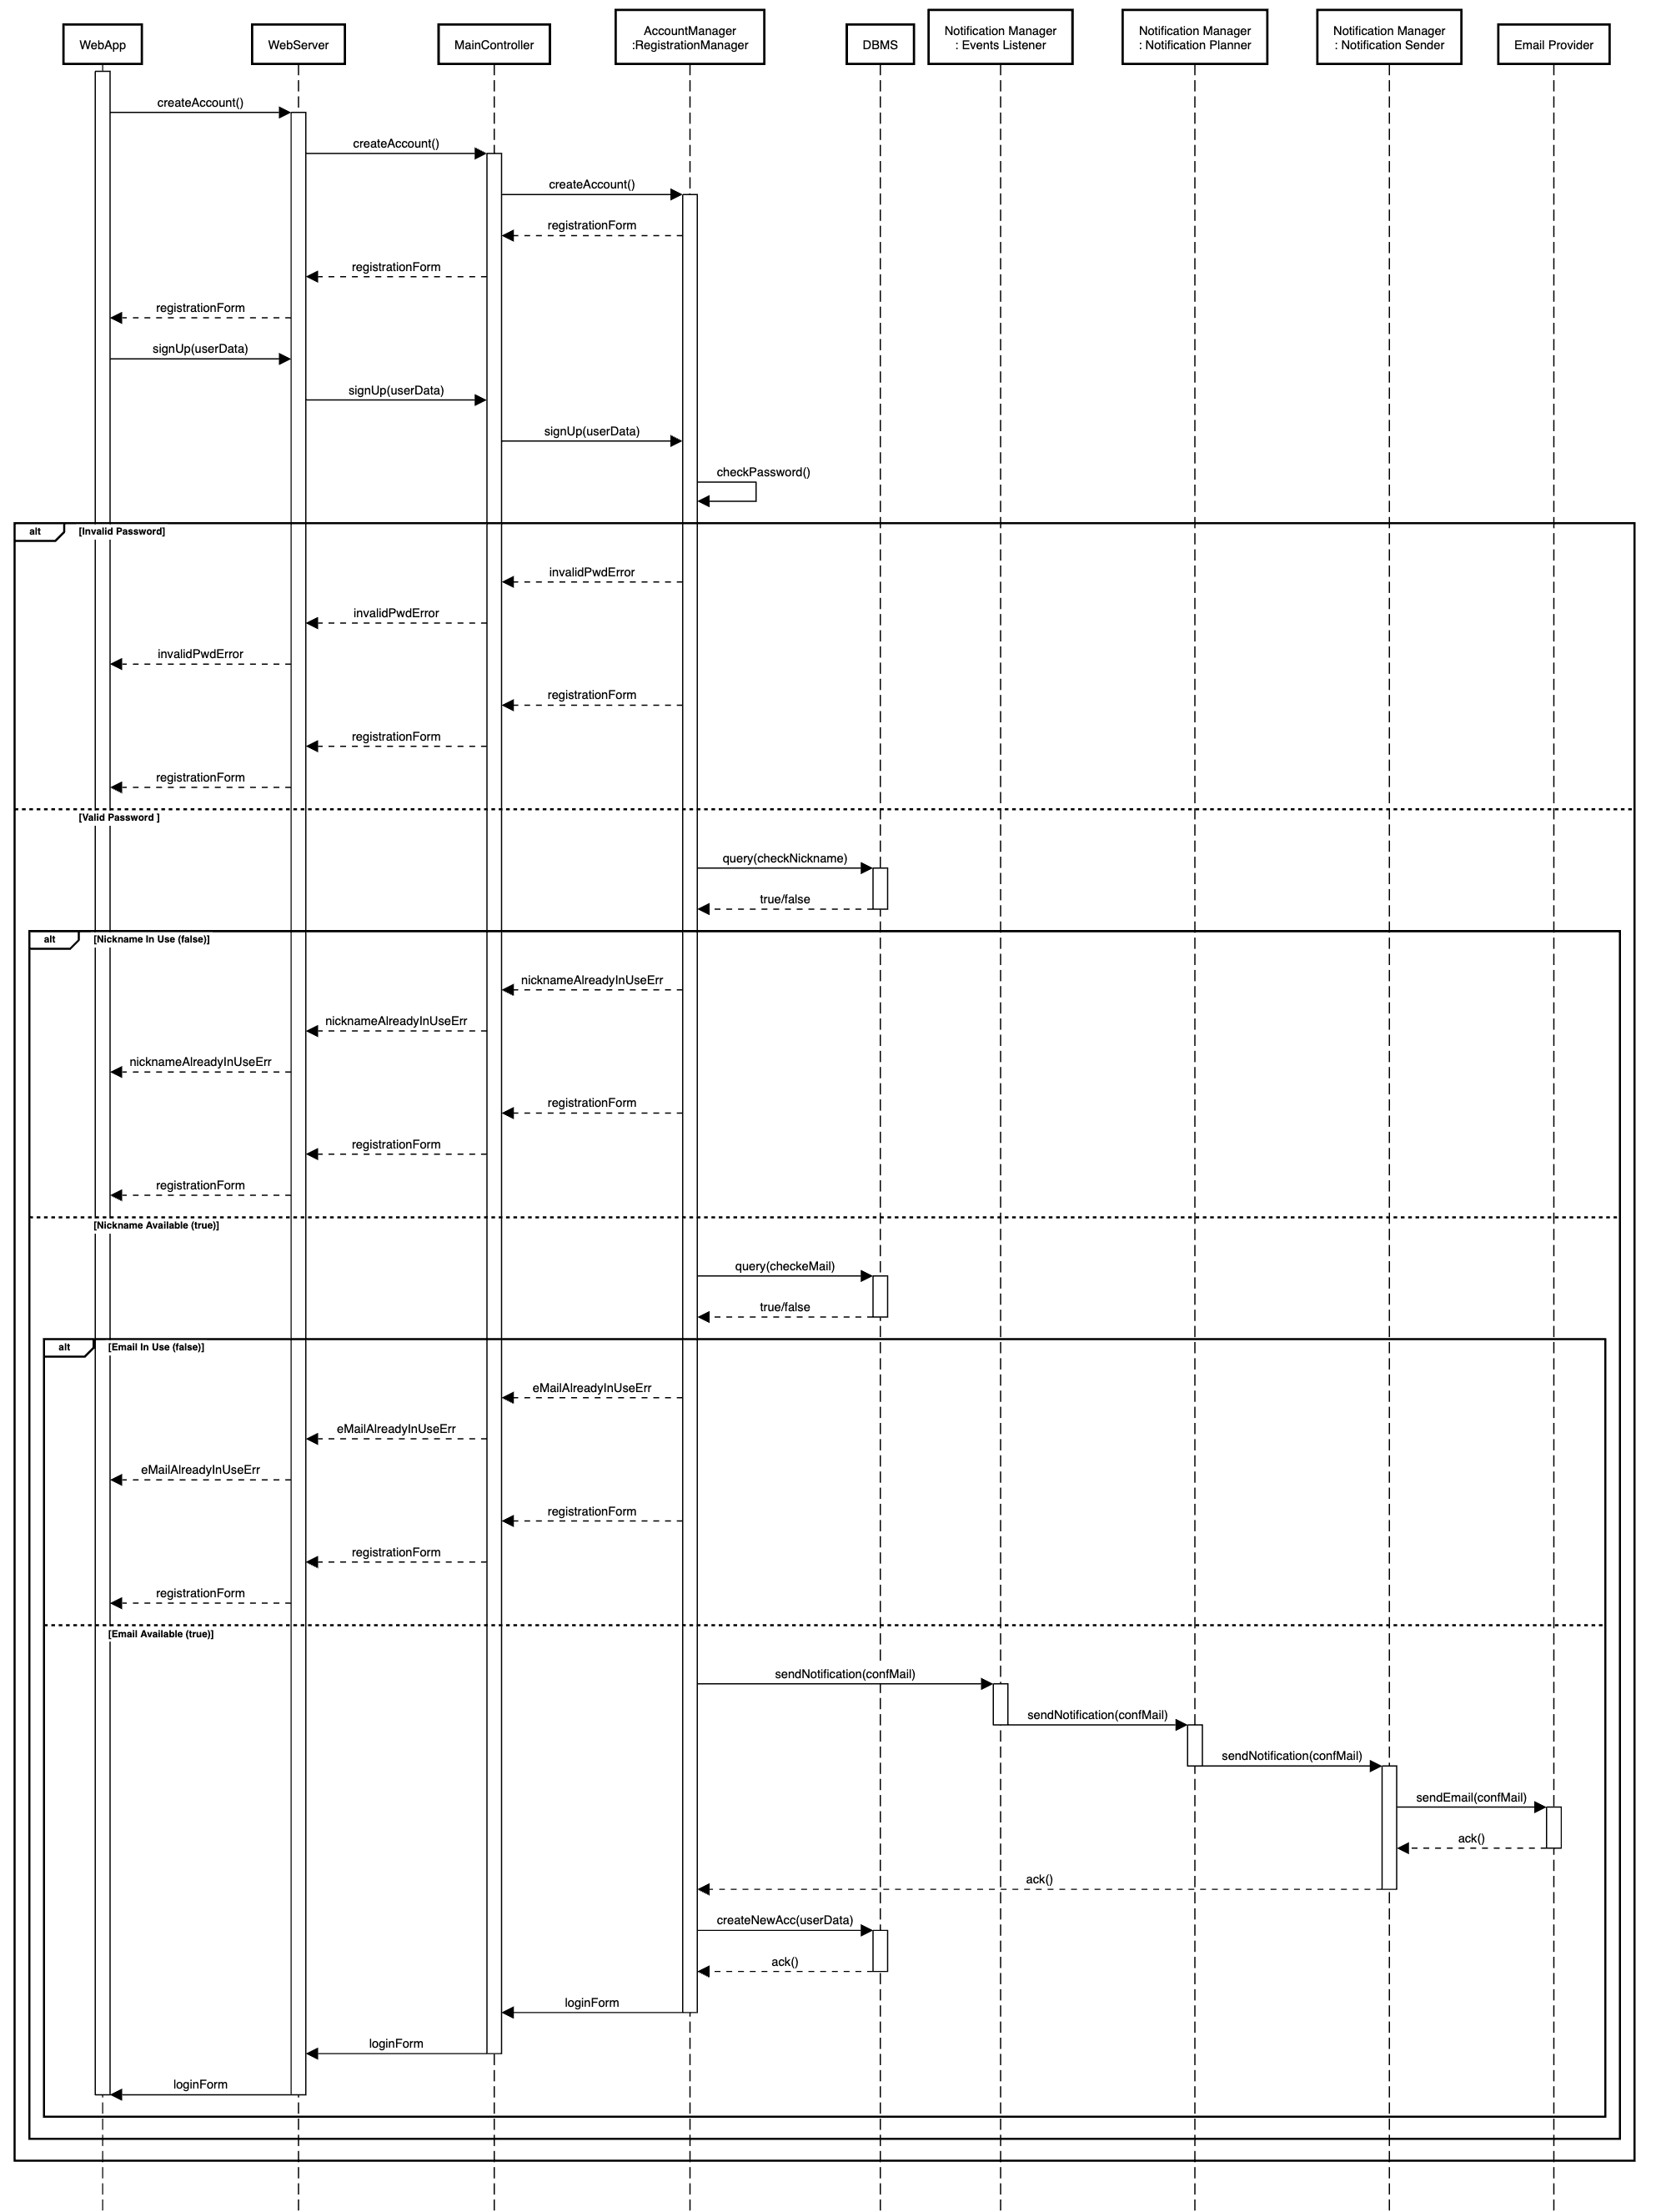
\includegraphics[width=\linewidth]{DD/Images/sequenceDiagrams/signUp.png}
    \caption{[UC1] Sign Up.}
    \label{fig:signUp_immagine}
\end{figure}

\clearpage
The sequence diagram outlines the sign-up process for students, companies, or universities. It starts with the user requesting an account through the WebApp, which retrieves a registration form via the WebServer and MainController. After the user submits their data, the RegistrationManager validates the password, username, and email by querying the database.

If any issues arise, such as an invalid password, duplicate username, or email, appropriate error messages are displayed, and the user is redirected to the registration form. Upon successful validation, the Notification Manager sends a confirmation email using the Email Provider. Finally, the RegistrationManager creates the account in the database and redirects the user to the login form, completing the process.

\begin{figure*}[htbp]
    \centering
    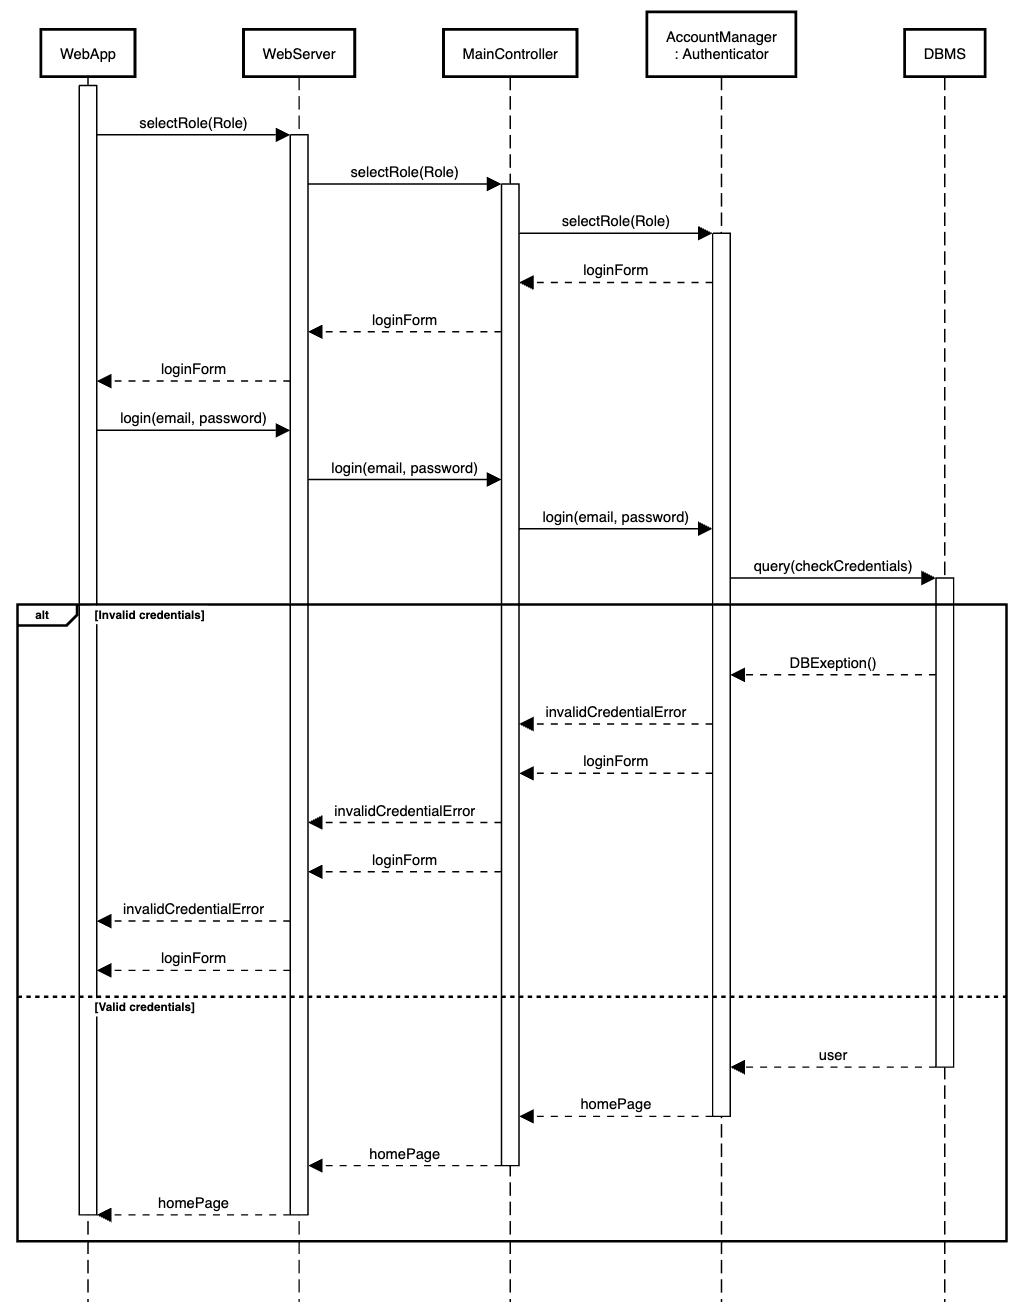
\includegraphics[width=\linewidth]{DD/Images/sequenceDiagrams/login.png}
    \caption{[UC2] Login.}
    \label{fig:login_immagine}
\end{figure*}
\clearpage

The sequence diagram outlines the login process: the user selects their role (student, company, or university) on the WebApp, triggering a request to the WebServer, which passes it to the MainController and then the Authenticator. The Authenticator retrieves the login form from the AccountManager and sends it back to the WebApp.

When the user submits their email and password, the WebApp forwards the credentials to the Authenticator, which verifies them with the database. If invalid, the Authenticator returns an error message via the WebServer and WebApp. If valid, the database sends the user’s information, and the Authenticator provides the home page. This ensures secure login validation and proper feedback.

\begin{figure*}[htbp]
    \centering
    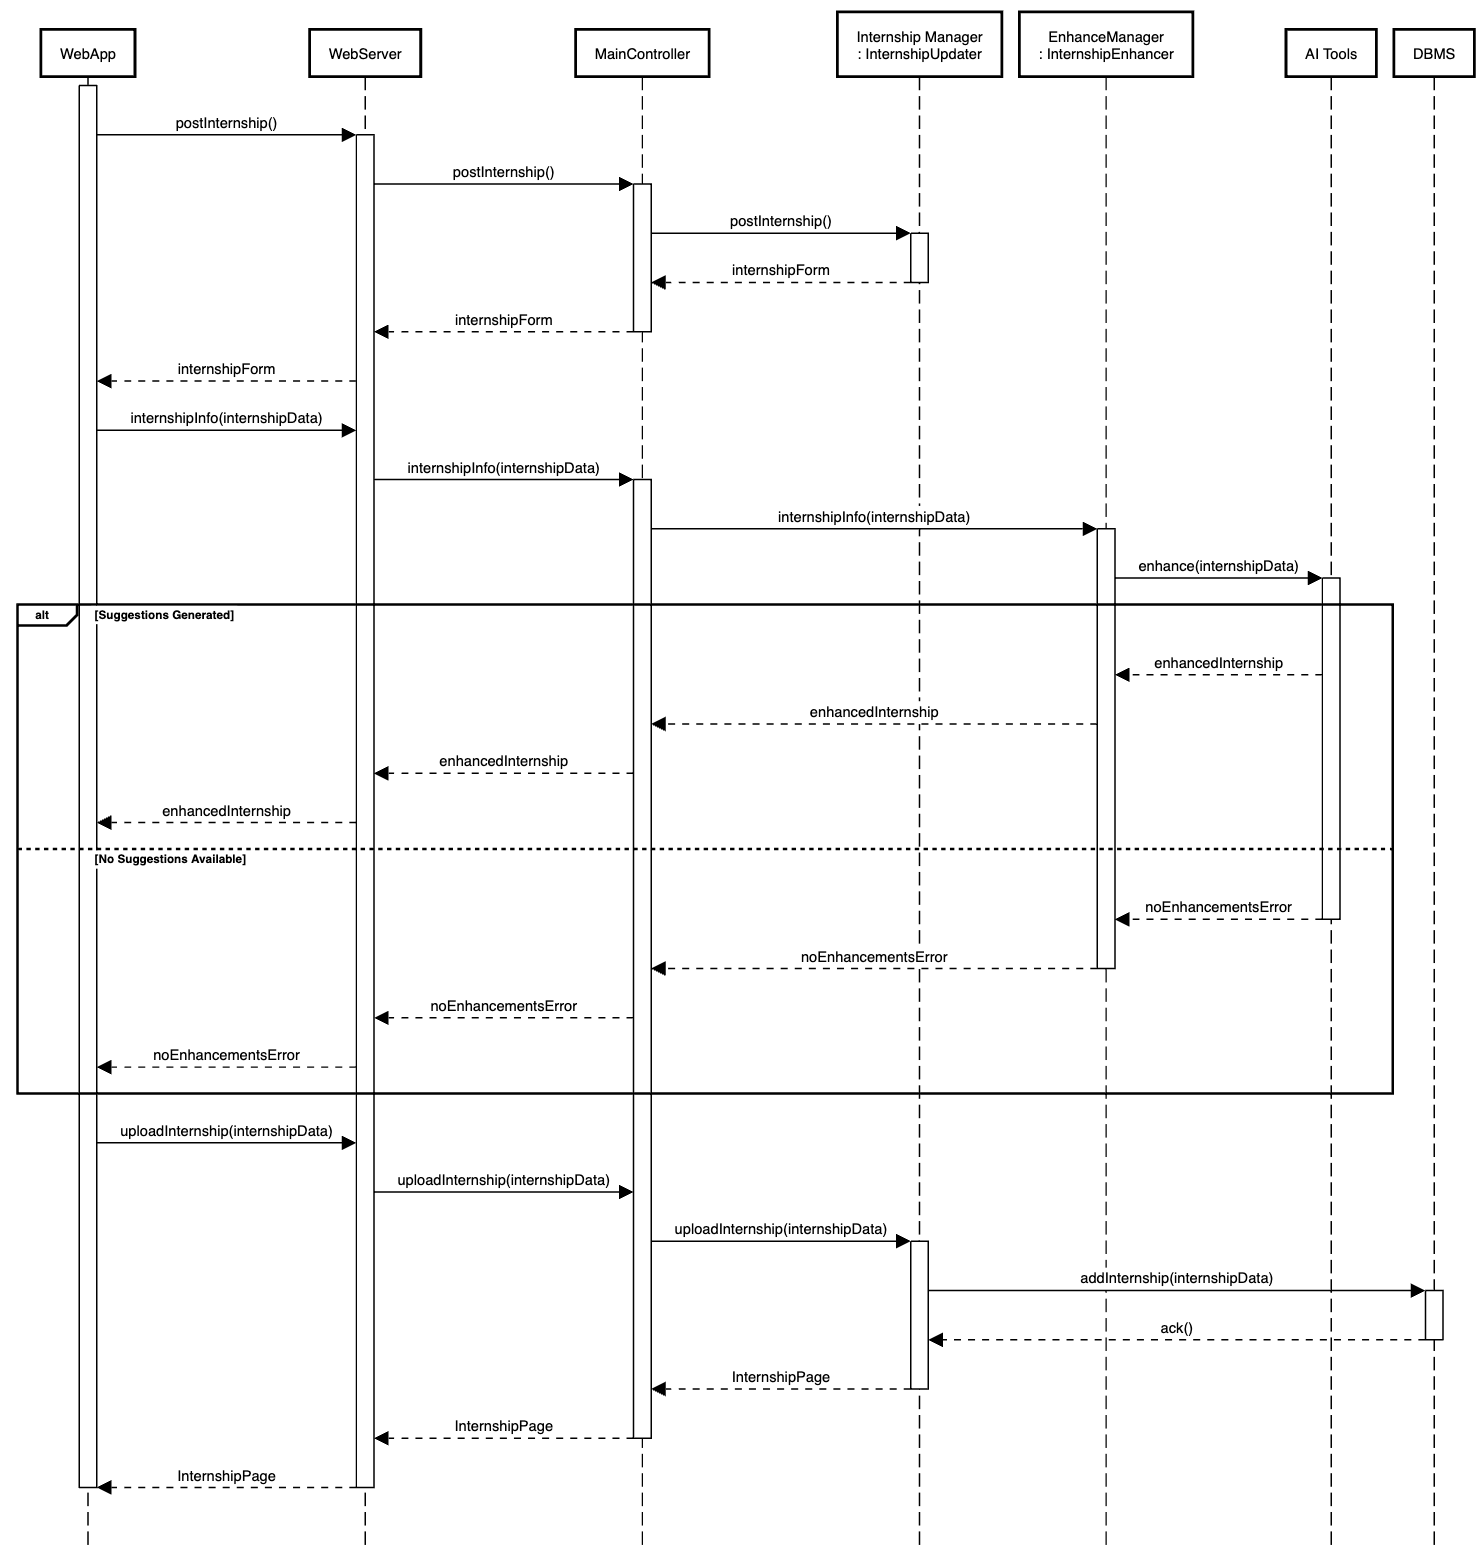
\includegraphics[width=\linewidth]{DD/Images/sequenceDiagrams/EhnanceInternship.png}
    \caption{[UC3] Insert Enhanced Internship Insertion.}
    \label{fig:enhanceInternship_immagine}
\end{figure*}
\clearpage

The sequence diagram illustrates the process of a Company, through the WebApp, inserting an enhanced internship. The process starts with the Company initiating a postInternship() request via the WebApp, which retrieves the internship form through the WebServer, MainController, and Internship Manager. The Company submits the internship data, which is enhanced by the EnhanceManager using AI Tools. If enhancements are available, they are returned to the WebApp; otherwise, an error message is sent.

After reviewing the enhancements, the Company uploads the internship data. This data is processed through the system and stored in the Database Management System. Once stored, an acknowledgment is sent back, and the Company, through the WebApp, receives the updated internship page as confirmation.

\begin{figure*}[htbp]
    \centering
    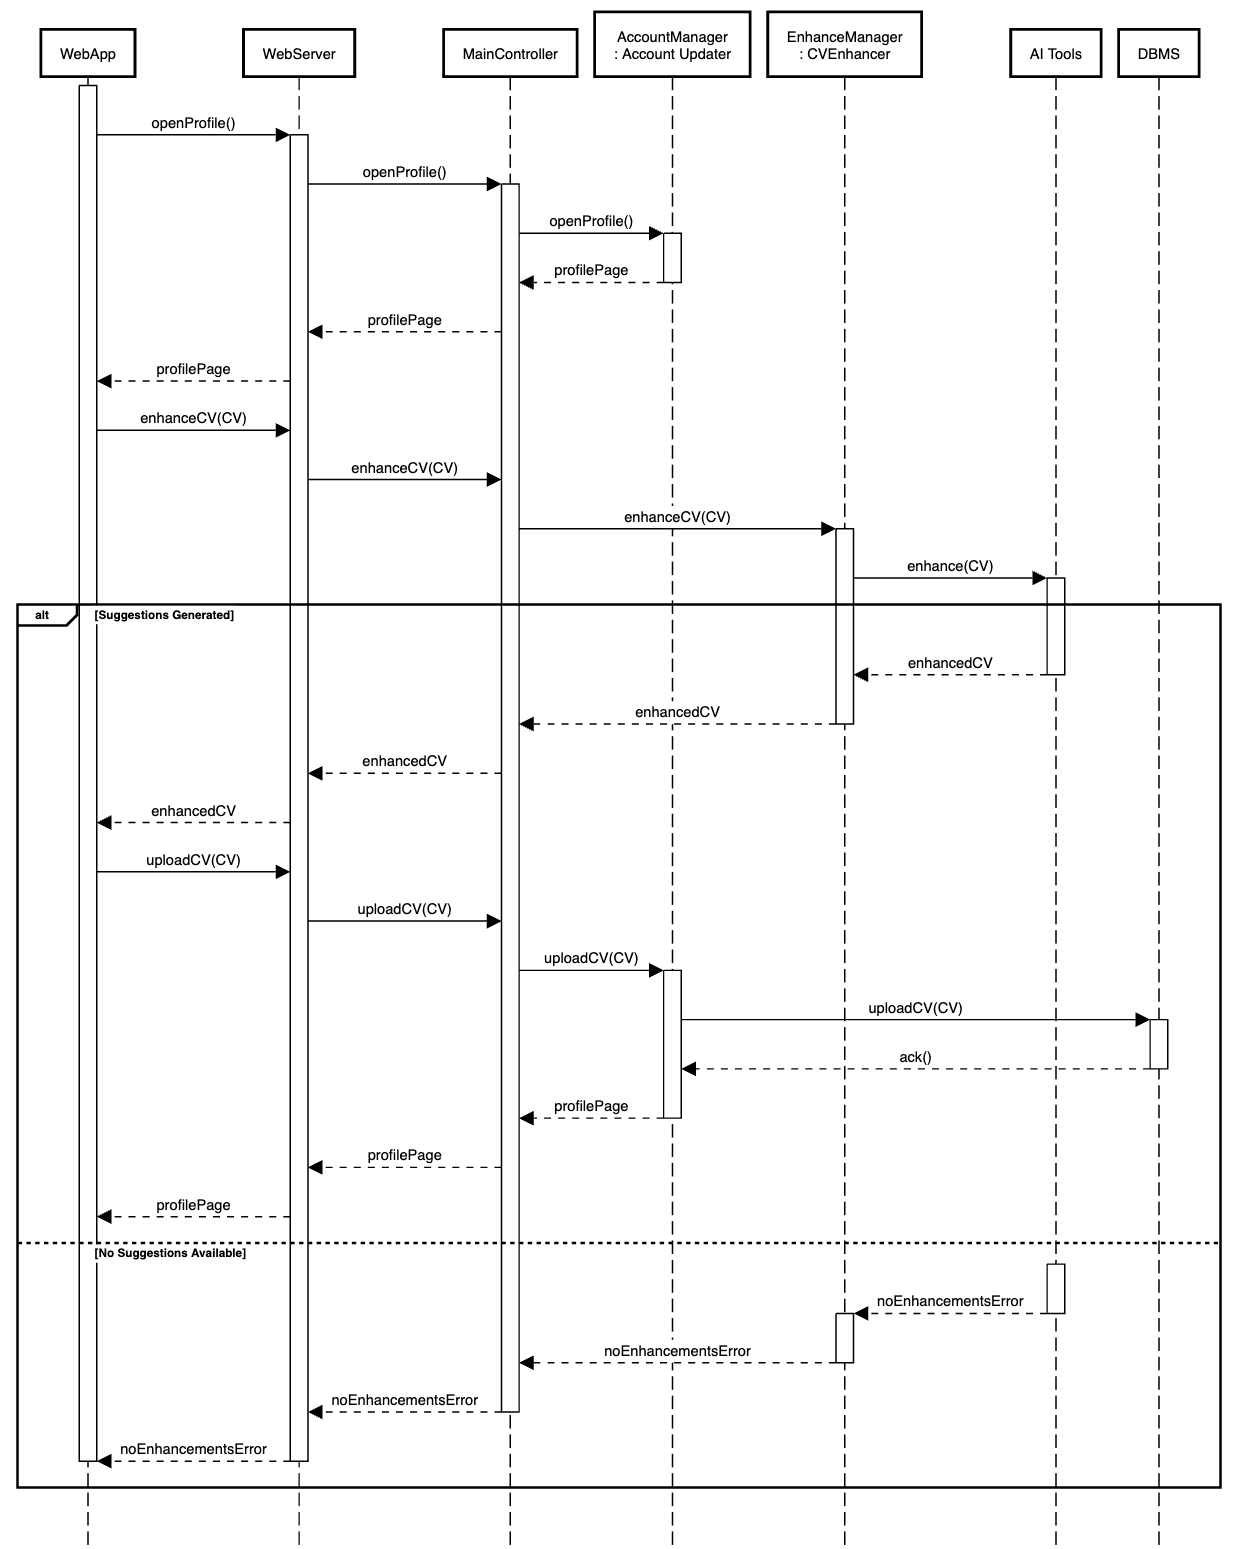
\includegraphics[width=\linewidth]{DD/Images/sequenceDiagrams/enhanceCV.png}
    \caption{[UC4] Enhance CV.}
    \label{fig:enhanceCV_immagine}
\end{figure*}
\clearpage

The sequence diagram illustrates the process of a Student enhancing their CV via the WebApp. The process starts with the Student sending an openProfile() request, which retrieves the profile page through the WebServer, MainController, and AccountManager. Once the profile page is loaded, the Student submits their CV for enhancement.

The CV is processed by the EnhanceManager using AI Tools. If enhancements are available, the enhanced CV is returned to the Student; otherwise, an error message is sent. After reviewing the enhancements, the Student uploads the updated CV. This CV is processed through the system and stored in the Database Management System. Finally, an acknowledgment is sent back, and the Student receives the updated profile page as confirmation.

\newpage

\begin{figure*}[htbp]
    \centering
    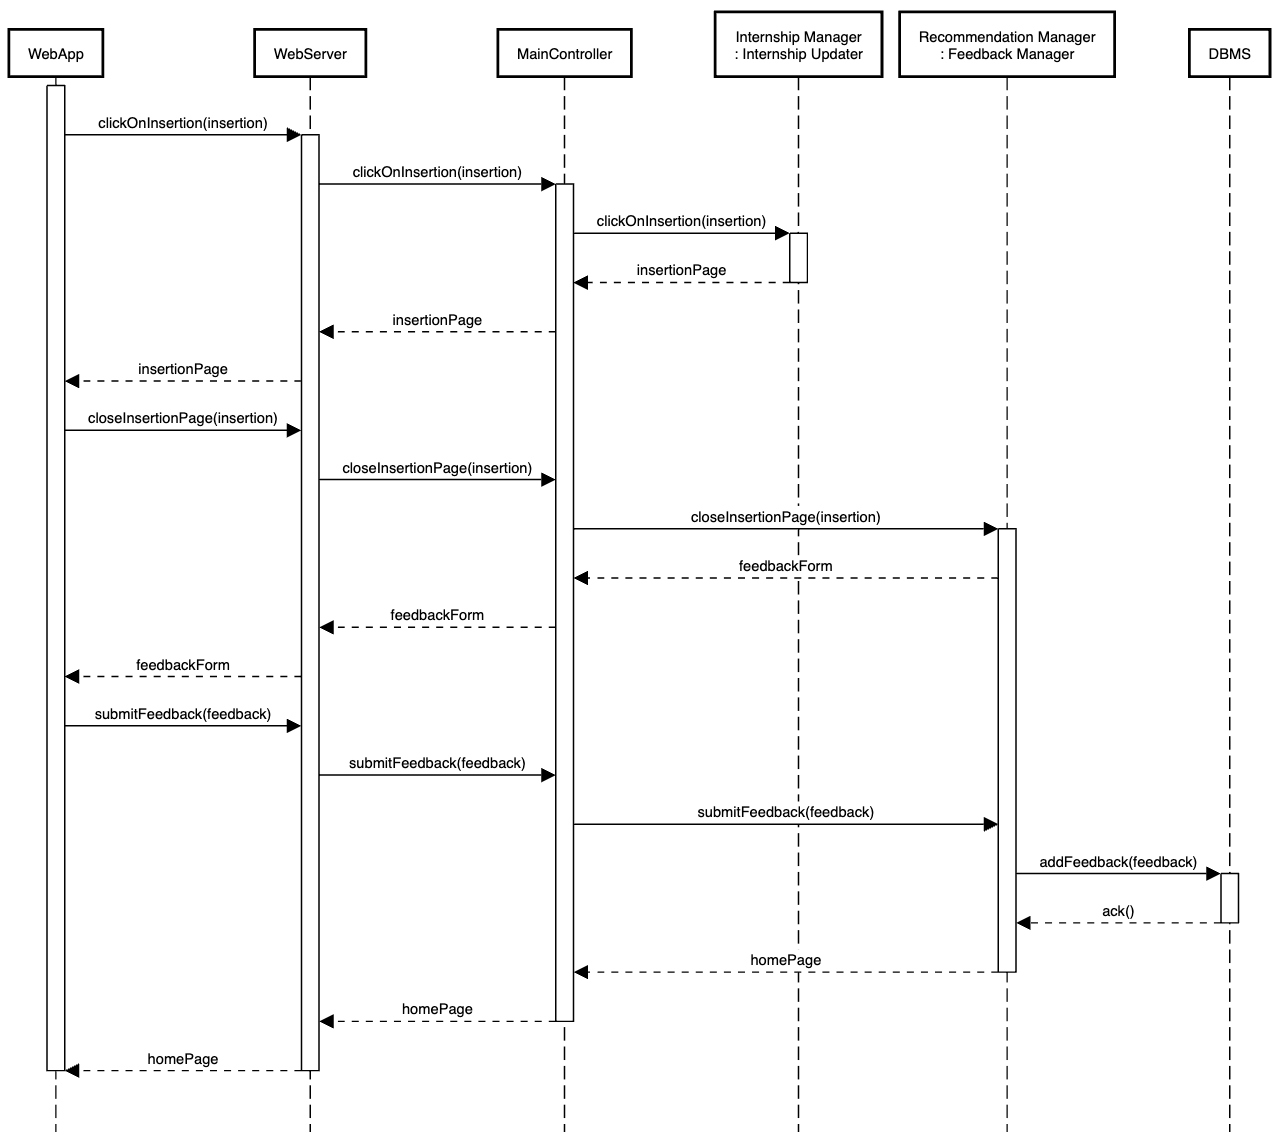
\includegraphics[width=\linewidth]{DD/Images/sequenceDiagrams/SubmitFeedback.png}
    \caption{[UC5] Submit a Feedback.}
    \label{fig:submitFeedback_immagine}
\end{figure*}


The sequence diagram illustrates the process of submitting feedback in the system. It begins with the user clicking on an insertion via the WebApp, which retrieves the insertion page through the WebServer, MainController, and Account Manager. After viewing the insertion, the user closes the insertion page, triggering the feedback process.

The WebApp requests a feedback form, which is generated by the Recommendation Manager and passed back through the system. The user submits their feedback via the WebApp, and it is processed through the WebServer, MainController, and Recommendation Manager. The feedback is stored in the Database Management System, where it will be used by the Data Analytics service to improve the recommendation engine in the future. Once stored, an acknowledgment is sent back, and the user is redirected to the home page as confirmation of successful feedback submission.

\begin{figure*}[htbp]
    \centering
    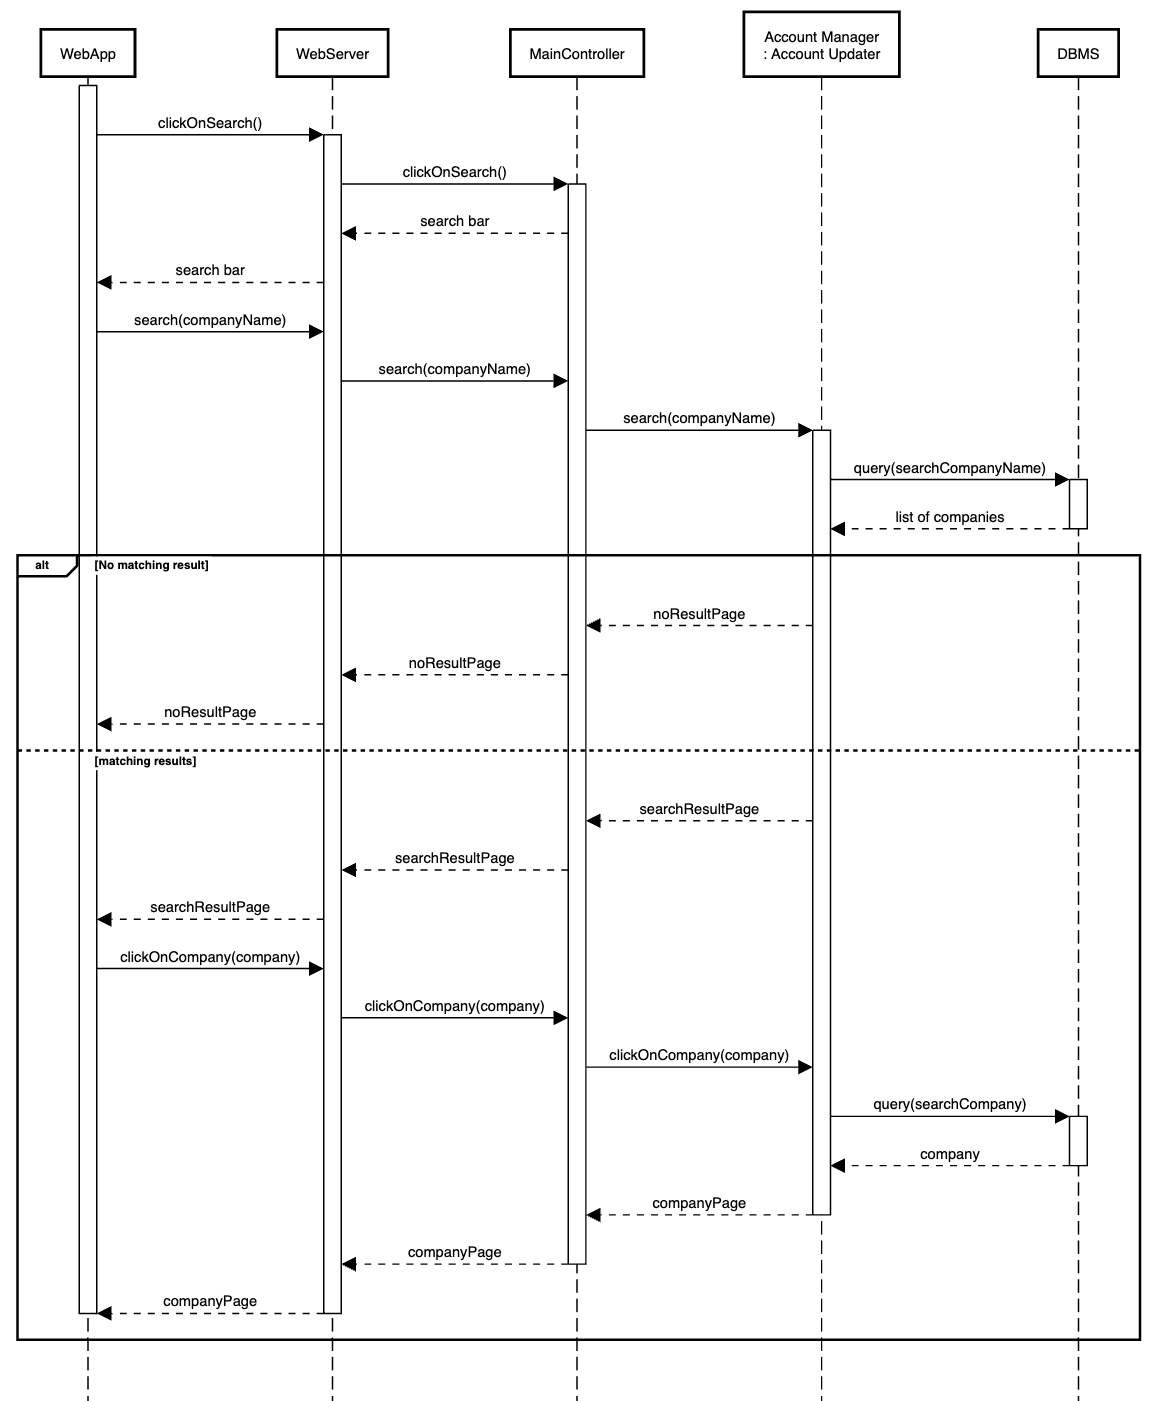
\includegraphics[width=\linewidth]{DD/Images/sequenceDiagrams/SearchCompany.png}
    \caption{[UC6] Search for a Company.}
    \label{fig:searchCompany_immagine}
\end{figure*}
\clearpage

The sequence diagram illustrates the process of searching for a company. It begins with the user initiating a search via the WebApp by clicking on the search option. This request is passed through the WebServer and MainController, which returns a search bar to the WebApp. The user enters the company name in the search bar, and the query is sent through the WebServer and MainController to the Account Manager.

The Account Manager queries the Database Management System for matching companies. If no results are found, a "no result" page is returned to the user. If matching results are found, a search result page is sent back.

The user can then click on a specific company from the results, triggering a request that is passed through the WebServer, MainController, and Account Manager. The Account Manager queries the database for the selected company's details, which are retrieved and sent back to the WebApp as a company page, completing the process.

\newpage

\begin{figure}[htbp]
    \centering
    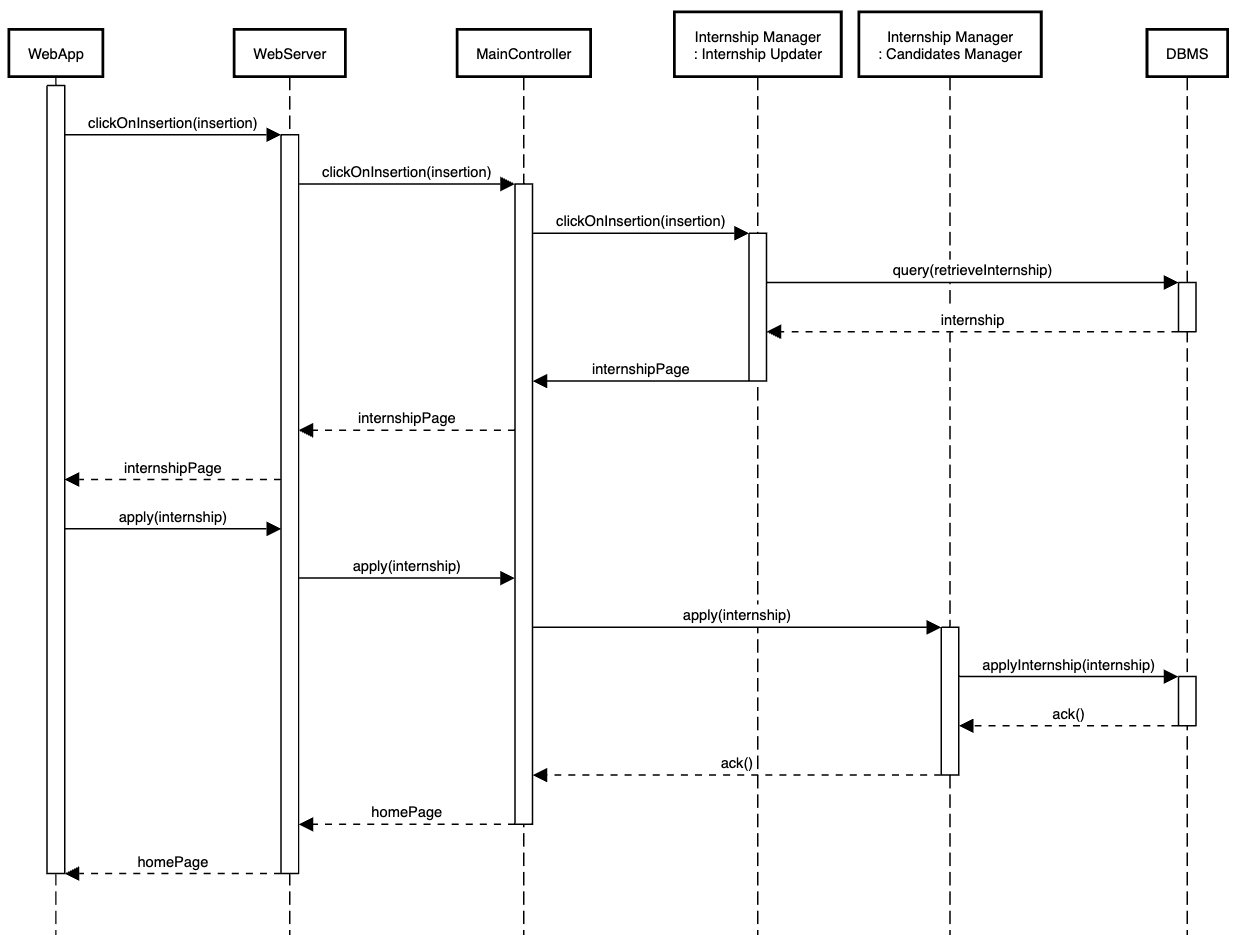
\includegraphics[width=\linewidth]{DD/Images/sequenceDiagrams/apply.png}
    \caption{[UC7] Apply for an Internship.}
    \label{fig:applyInternship_immagine}
\end{figure}

The sequence diagram shows the process of a student applying for an internship through the S\&C application. The student clicks on an internship insertion in the WebApp, which sends a request to the WebServer and MainController to retrieve the internship details from the database. 

After reviewing the internship, the student clicks "apply," which triggers the MainController to forward the application to the Candidates Manager. The Candidates Manager updates the database, and once the application is acknowledged, the MainController sends the student back to the home page, which is displayed on the WebApp.

\begin{figure*}[htbp]
    \centering
    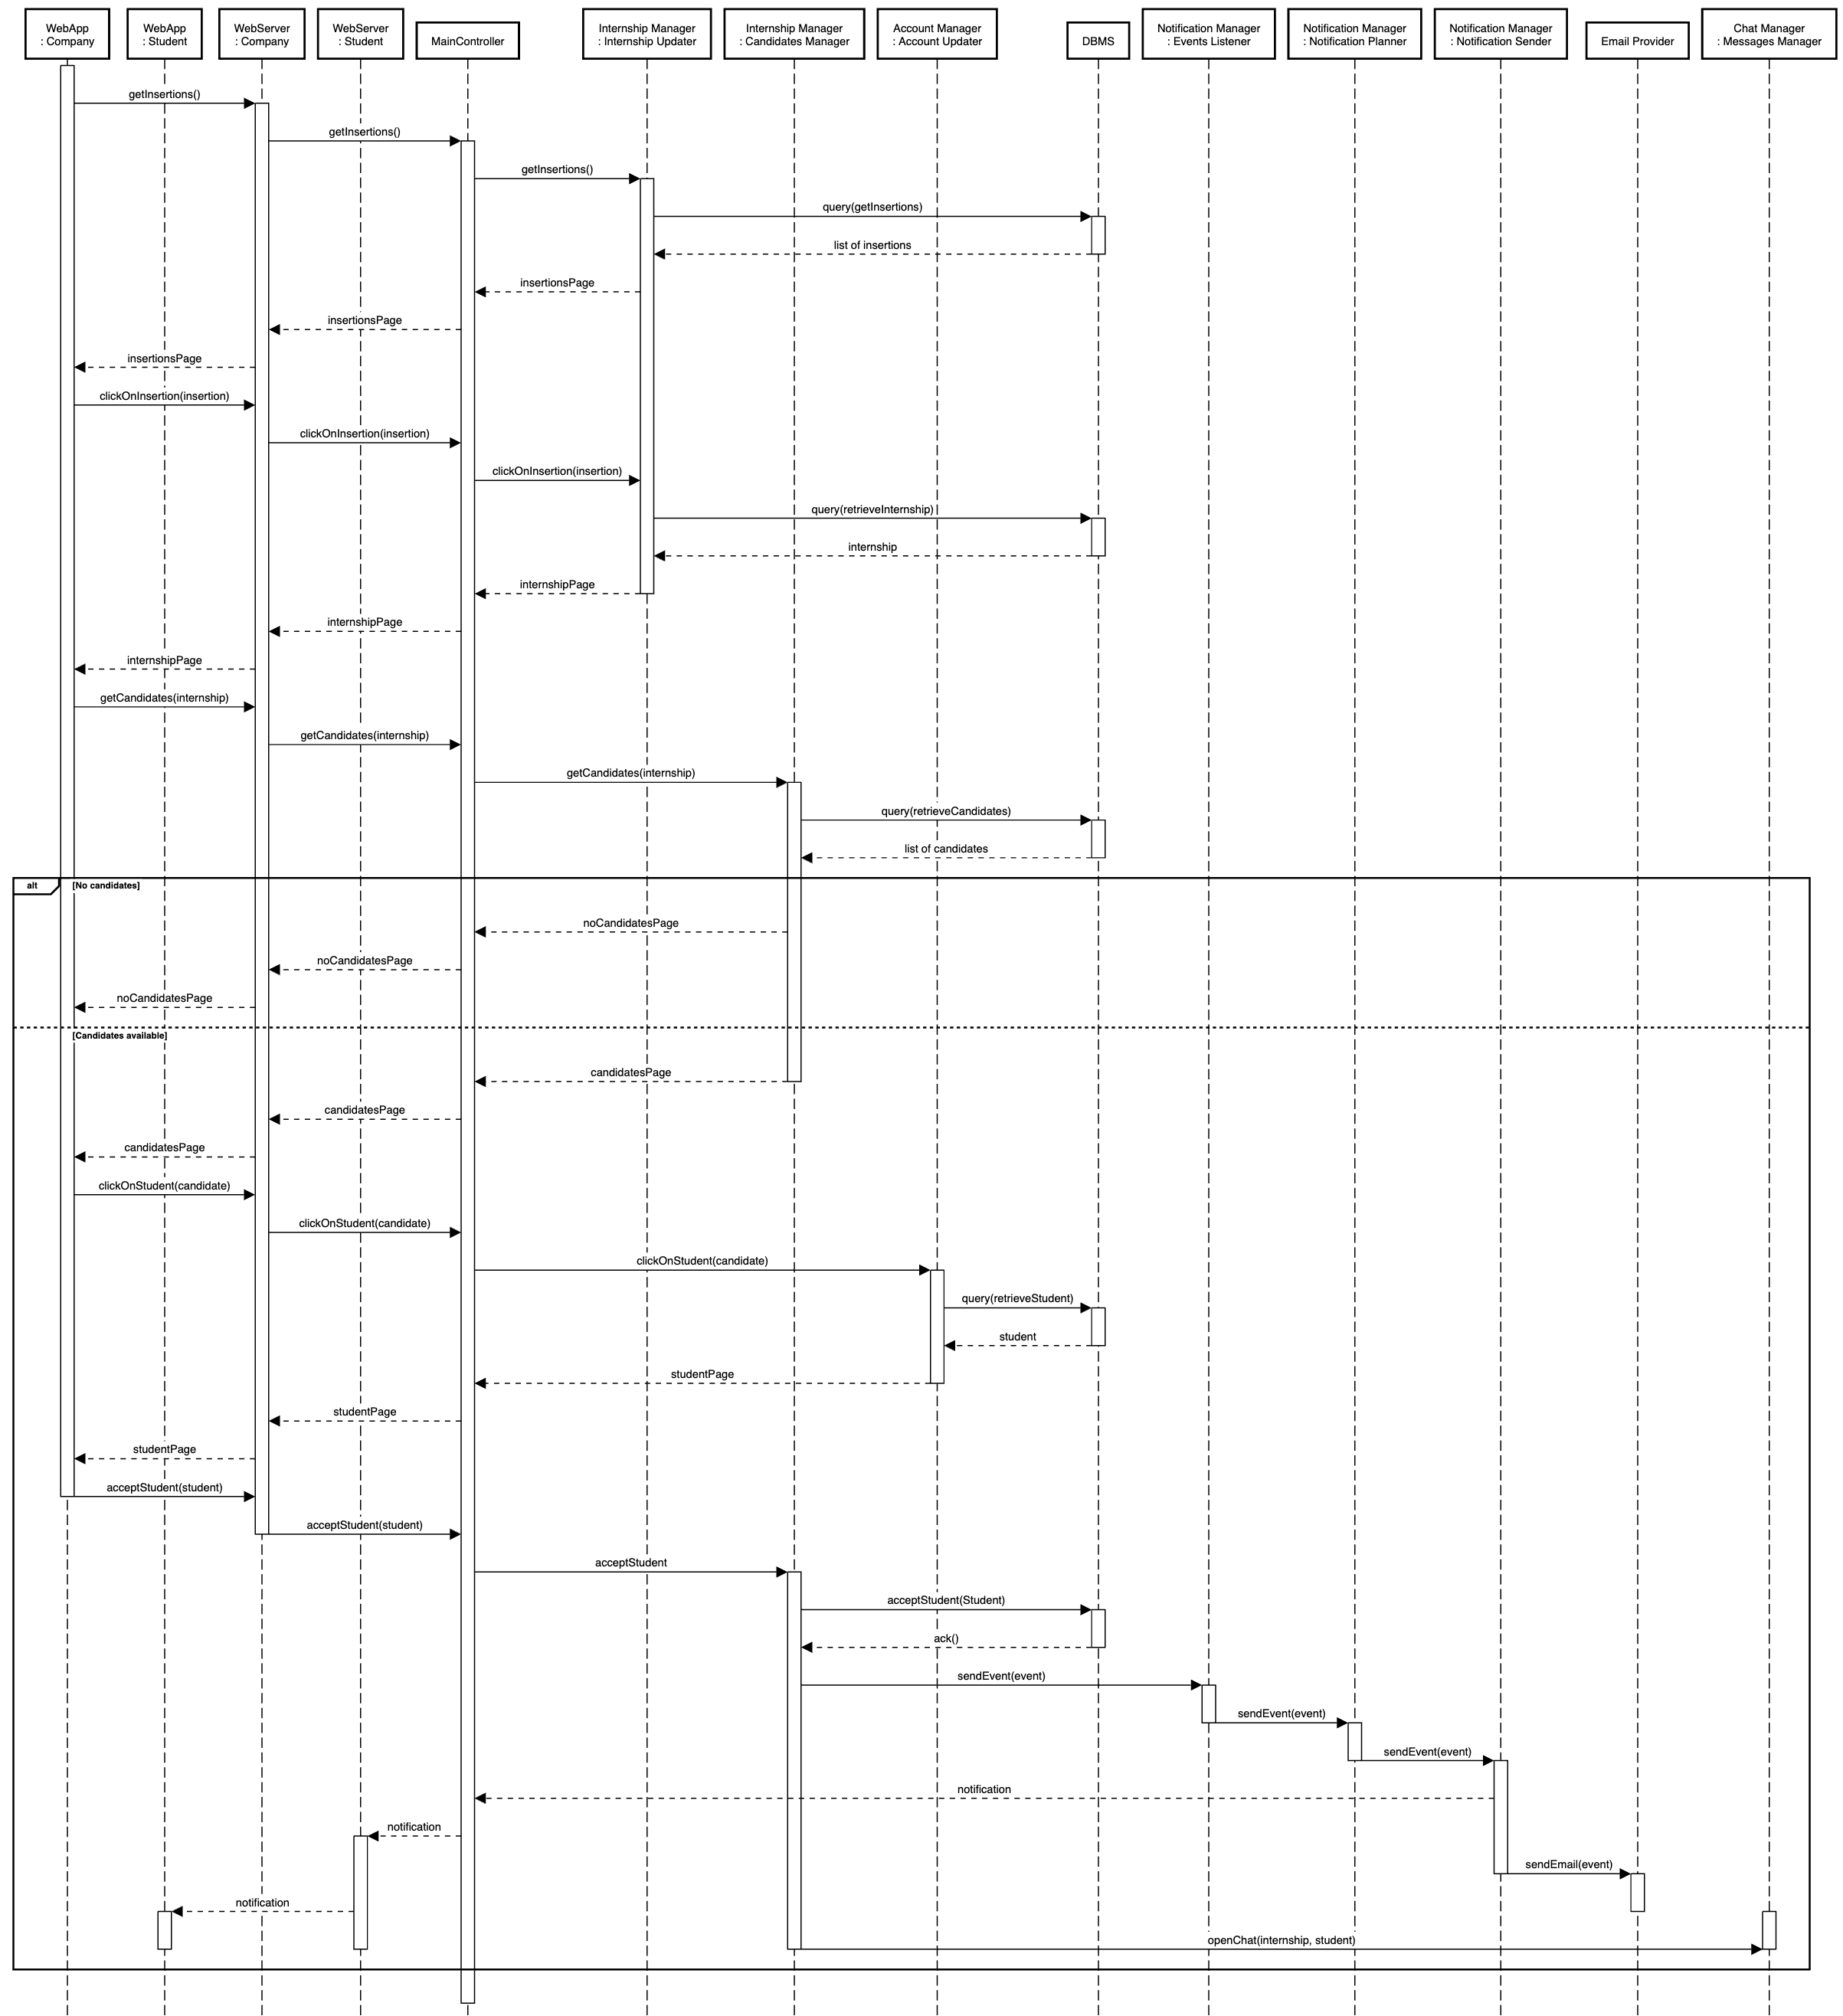
\includegraphics[width=\linewidth]{DD/Images/sequenceDiagrams/AcceptCandidate.png}
    \caption{[UC8] Accept a Candidate.}
    \label{fig:acceptCandidate_immagine}
\end{figure*}
\clearpage


The sequence diagram depicts the process of a company accepting a candidate for an internship. The company first retrieves a list of internship insertions, which are the internships they are offering. After selecting an internship, the company requests the list of candidates who have applied for it. If candidates are available, the company scrolls through the list and clicks on a candidate's profile to view their details. The system retrieves the student's information and displays it.

Once the company decides to accept the candidate, the action is processed by the MainController, which updates the database and triggers notifications. The student is notified through the WebApp and via email. Additionally, a chat is opened between the company and the student for further communication.

\begin{figure*}[htbp]
    \centering
    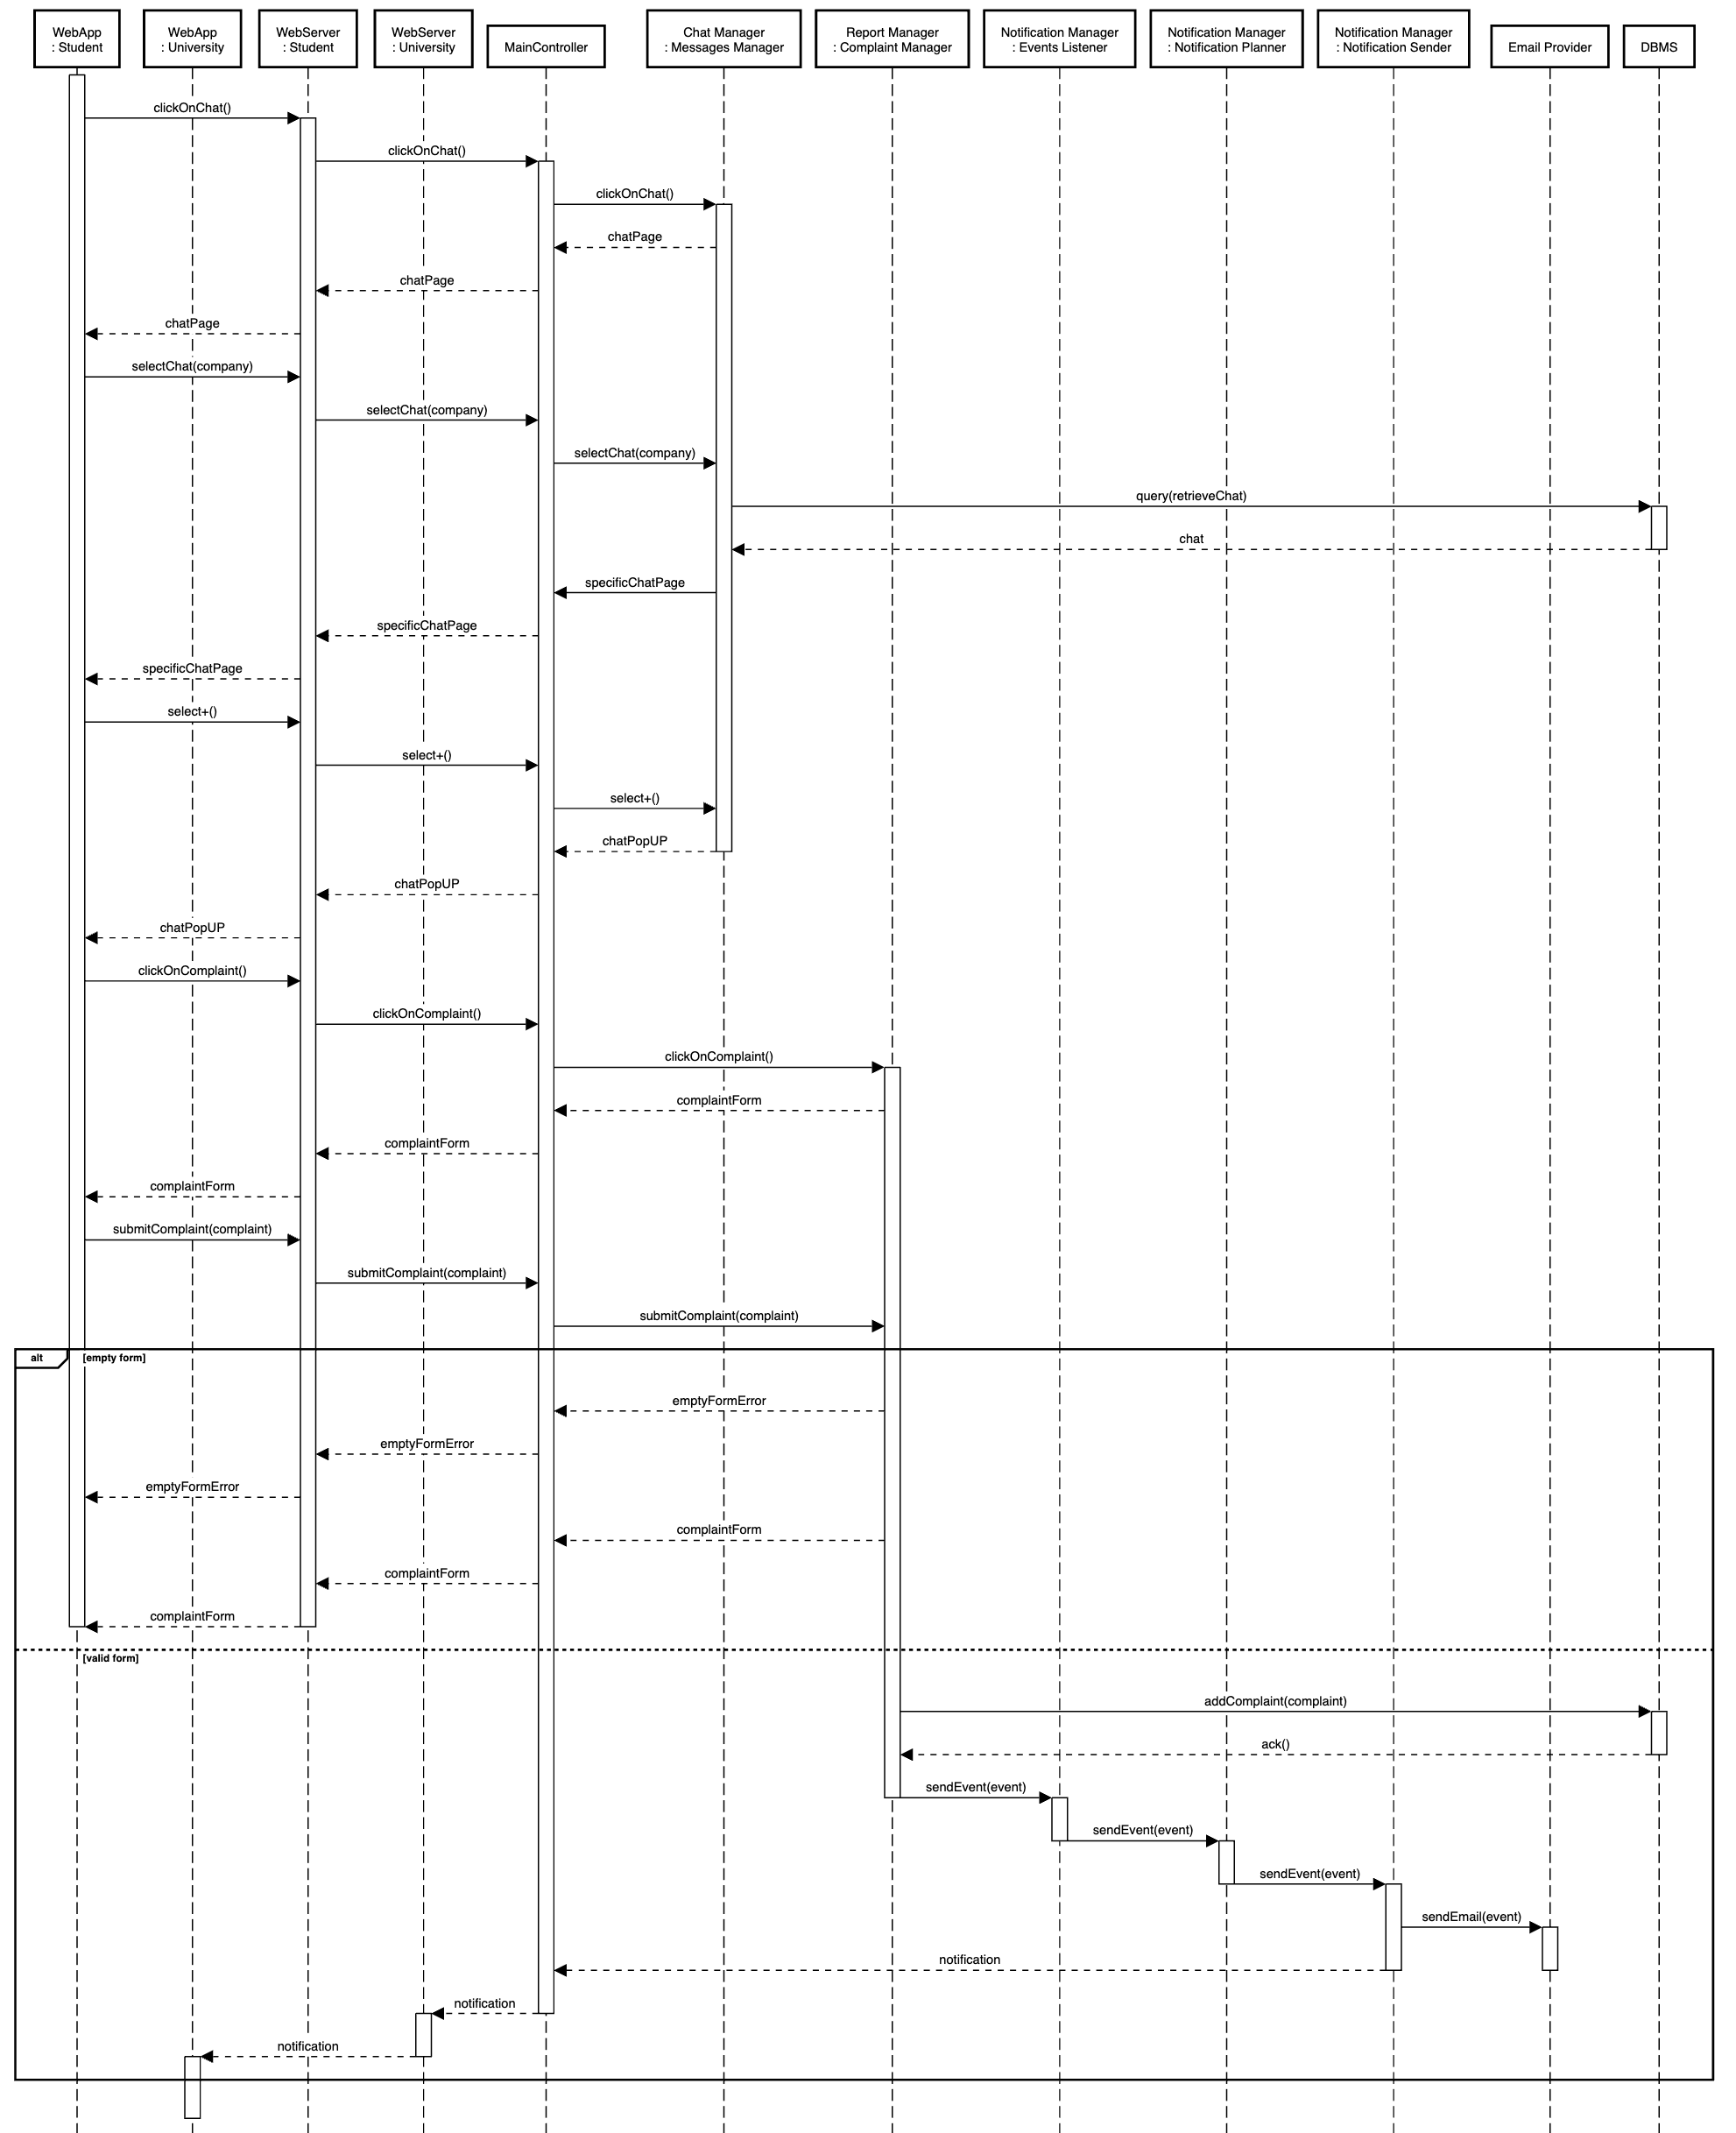
\includegraphics[width=\linewidth]{DD/Images/sequenceDiagrams/sumbitComplaint.png}
    \caption{[UC9] Submit a Complaint.}
    \label{fig:submitComplaint_immagine}
\end{figure*}
\clearpage

The sequence diagram illustrates the process of a student submitting a complaint through the S\&C application. The student first clicks on the chat logo in the WebApp, which opens the chat page. The WebServer retrieves and displays the chat page. The student then selects the specific chat with the company, and the system displays the chat details.

Next, the student clicks on the "+" logo, which opens a popup with various options, one of which is the "complaint" option. After selecting "complaint," the system presents the complaint form. The student fills it out and submits it. If the form is empty, an error is shown, prompting the student to complete it. Once the student submits a valid complaint, the Complaint Manager adds it to the database, and the system acknowledges the action.

The Complaint Manager triggers an event, which is processed by the Notification Manager. The event is passed through the Notification Planner and Notification Sender, which sends an email to the relevant parties, including the student's university. The university is notified about the complaint, completing the process for the student.

This same process can also be performed by the company. The company can submit a complaint in the same way, by selecting the chat and submitting a problem, which is processed similarly.

\begin{figure*}[htbp]
    \centering
    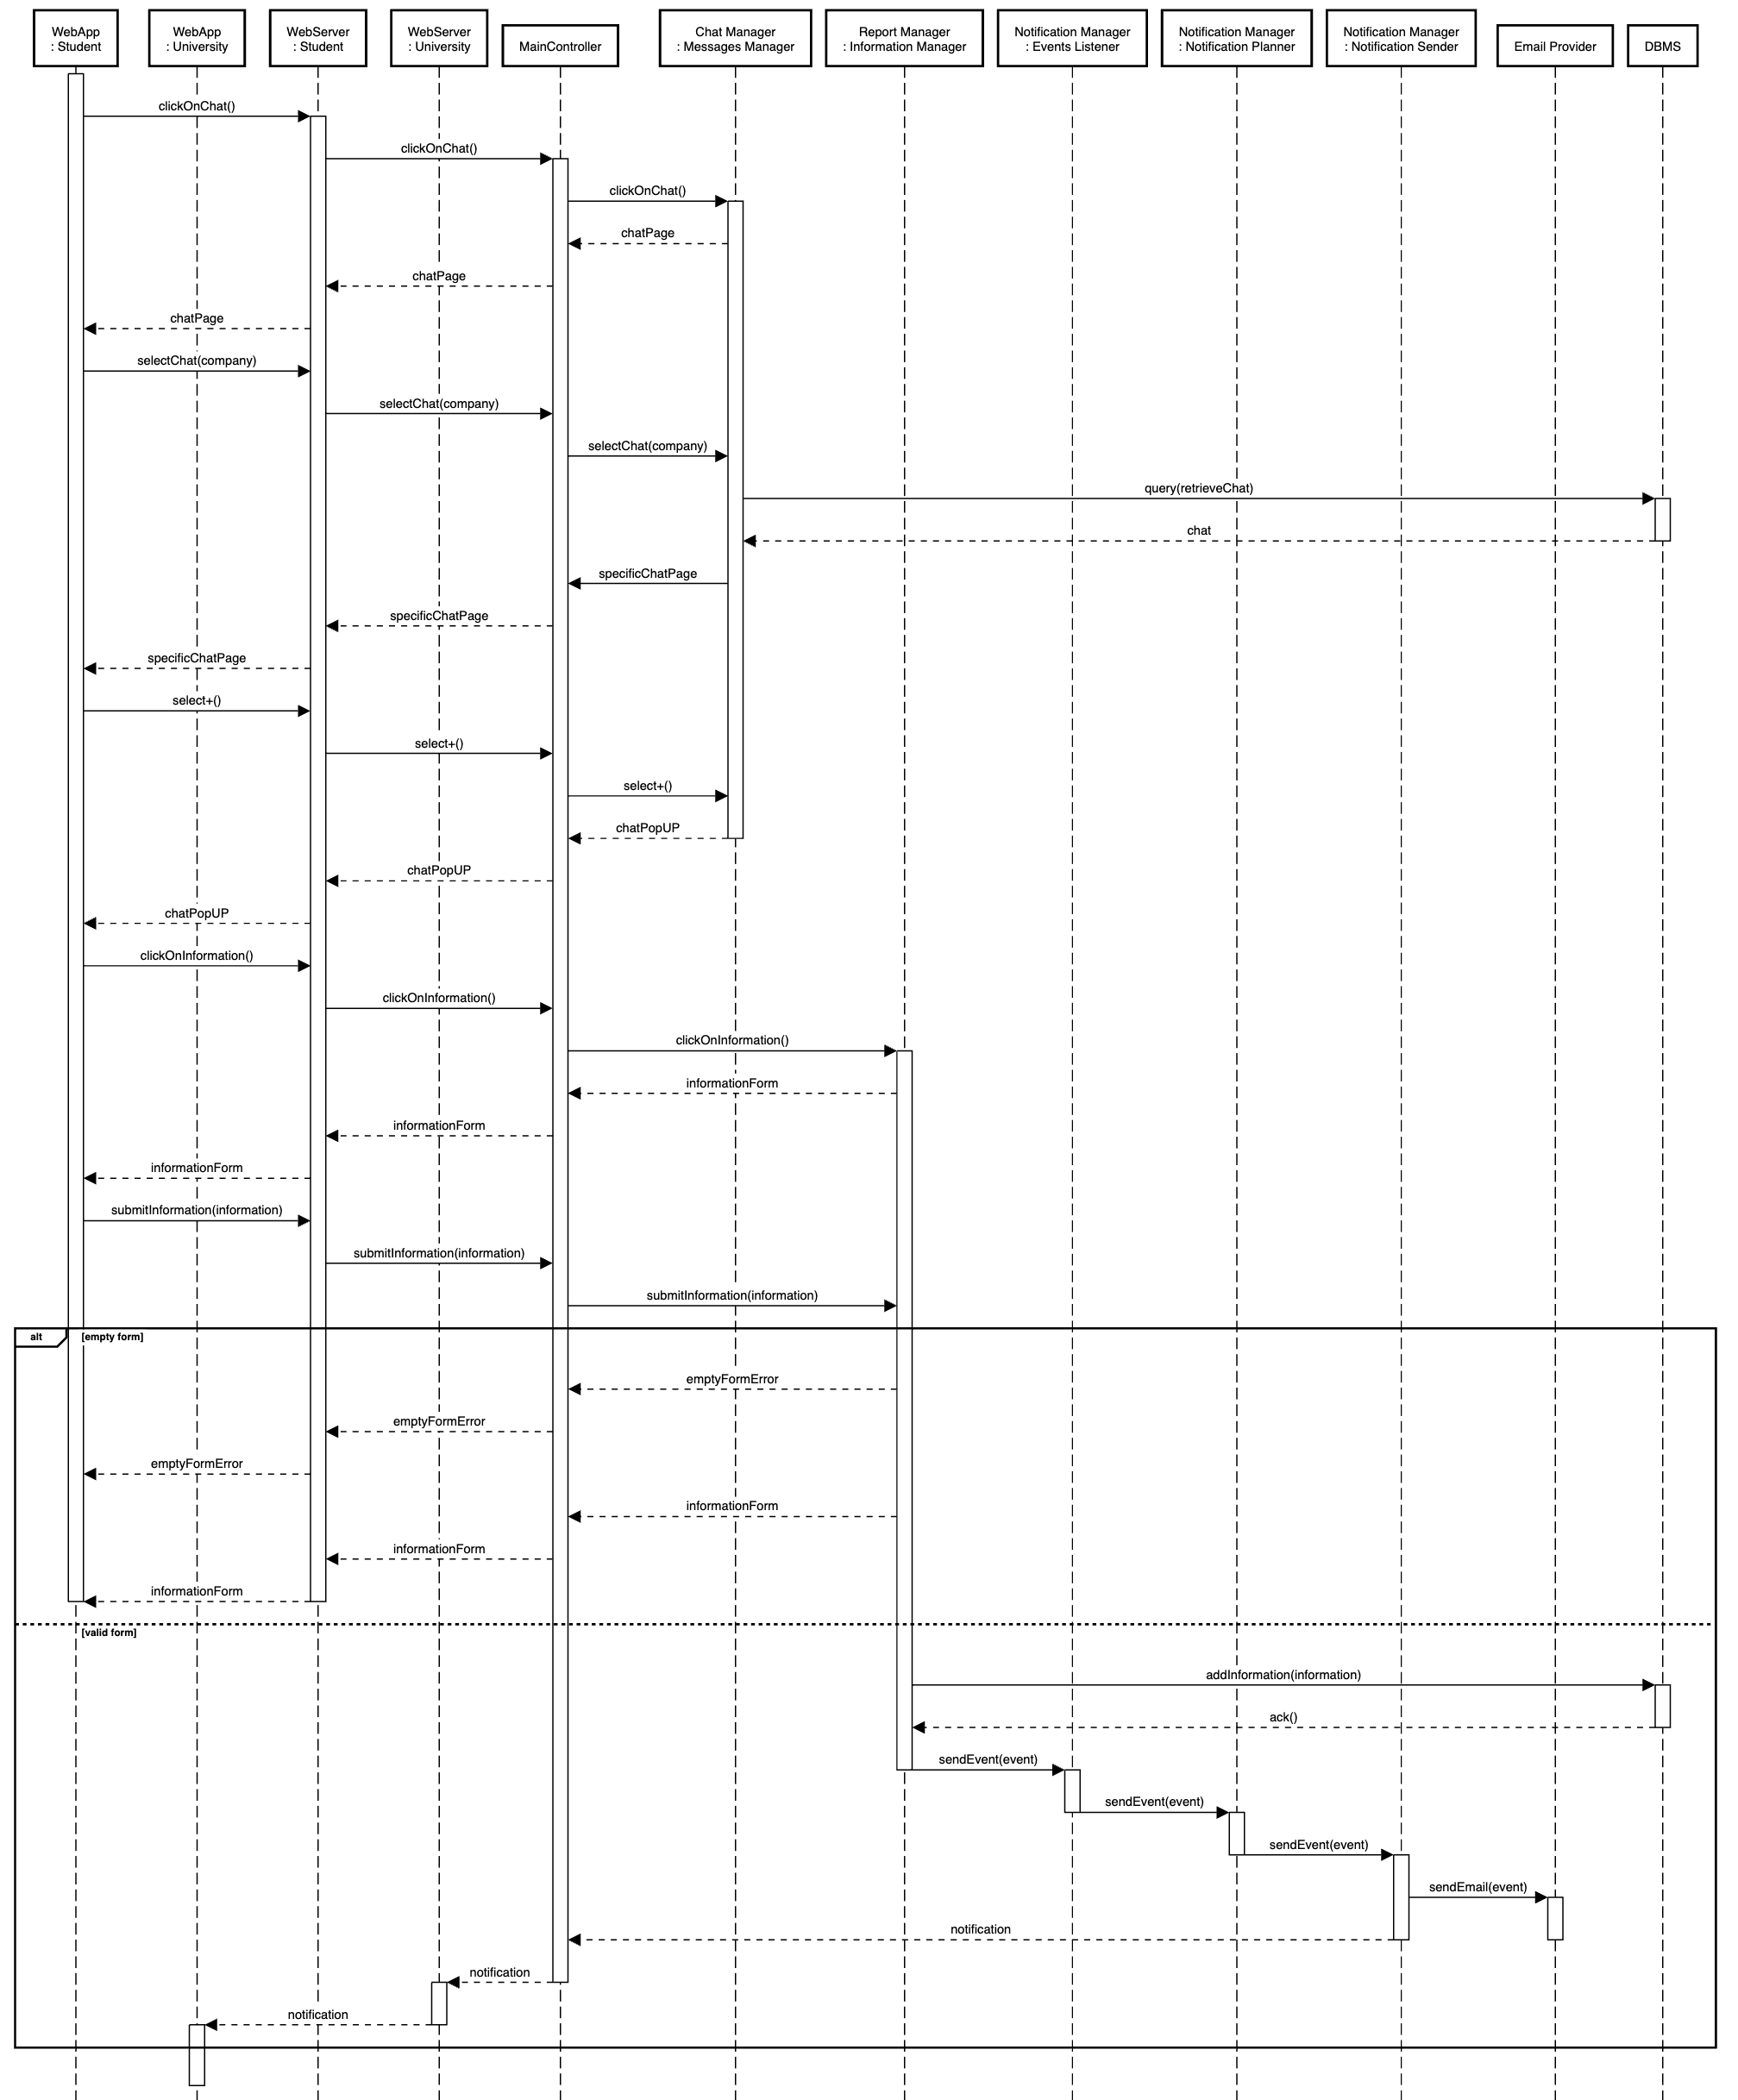
\includegraphics[width=\linewidth]{DD/Images/sequenceDiagrams/submitInformation.png}
    \caption{[UC10] Submit an Information.}
    \label{fig:submitInformation_immagine}
\end{figure*}
\clearpage

The sequence diagram illustrates the process of a student submitting an information report through the S\&C application. The student first clicks on the chat logo in the WebApp, which opens the chat page. The WebServer retrieves and displays the chat page. The student then selects the specific chat with the company, and the system displays the chat details.

Next, the student clicks on the "+" logo, which opens a popup with various options, one of which is the "information" option. After selecting "information," the system presents the information form. The student fills out the form and submits it. If the form is empty, an error is shown, prompting the student to complete it. Once the student submits a valid report, the Information Manager adds it to the database, and the system acknowledges the action.

The Information Manager triggers an event, which is processed by the Notification Manager. The event is passed through the Notification Planner and Notification Sender, which sends an email to the relevant parties, including the student's university. The university is notified about the information report, completing the process for the student.

This same process can also be performed by the company. The company can submit an information report in the same way, by selecting the chat and submitting the information, which is processed similarly.

\begin{figure*}[htbp]
    \centering
    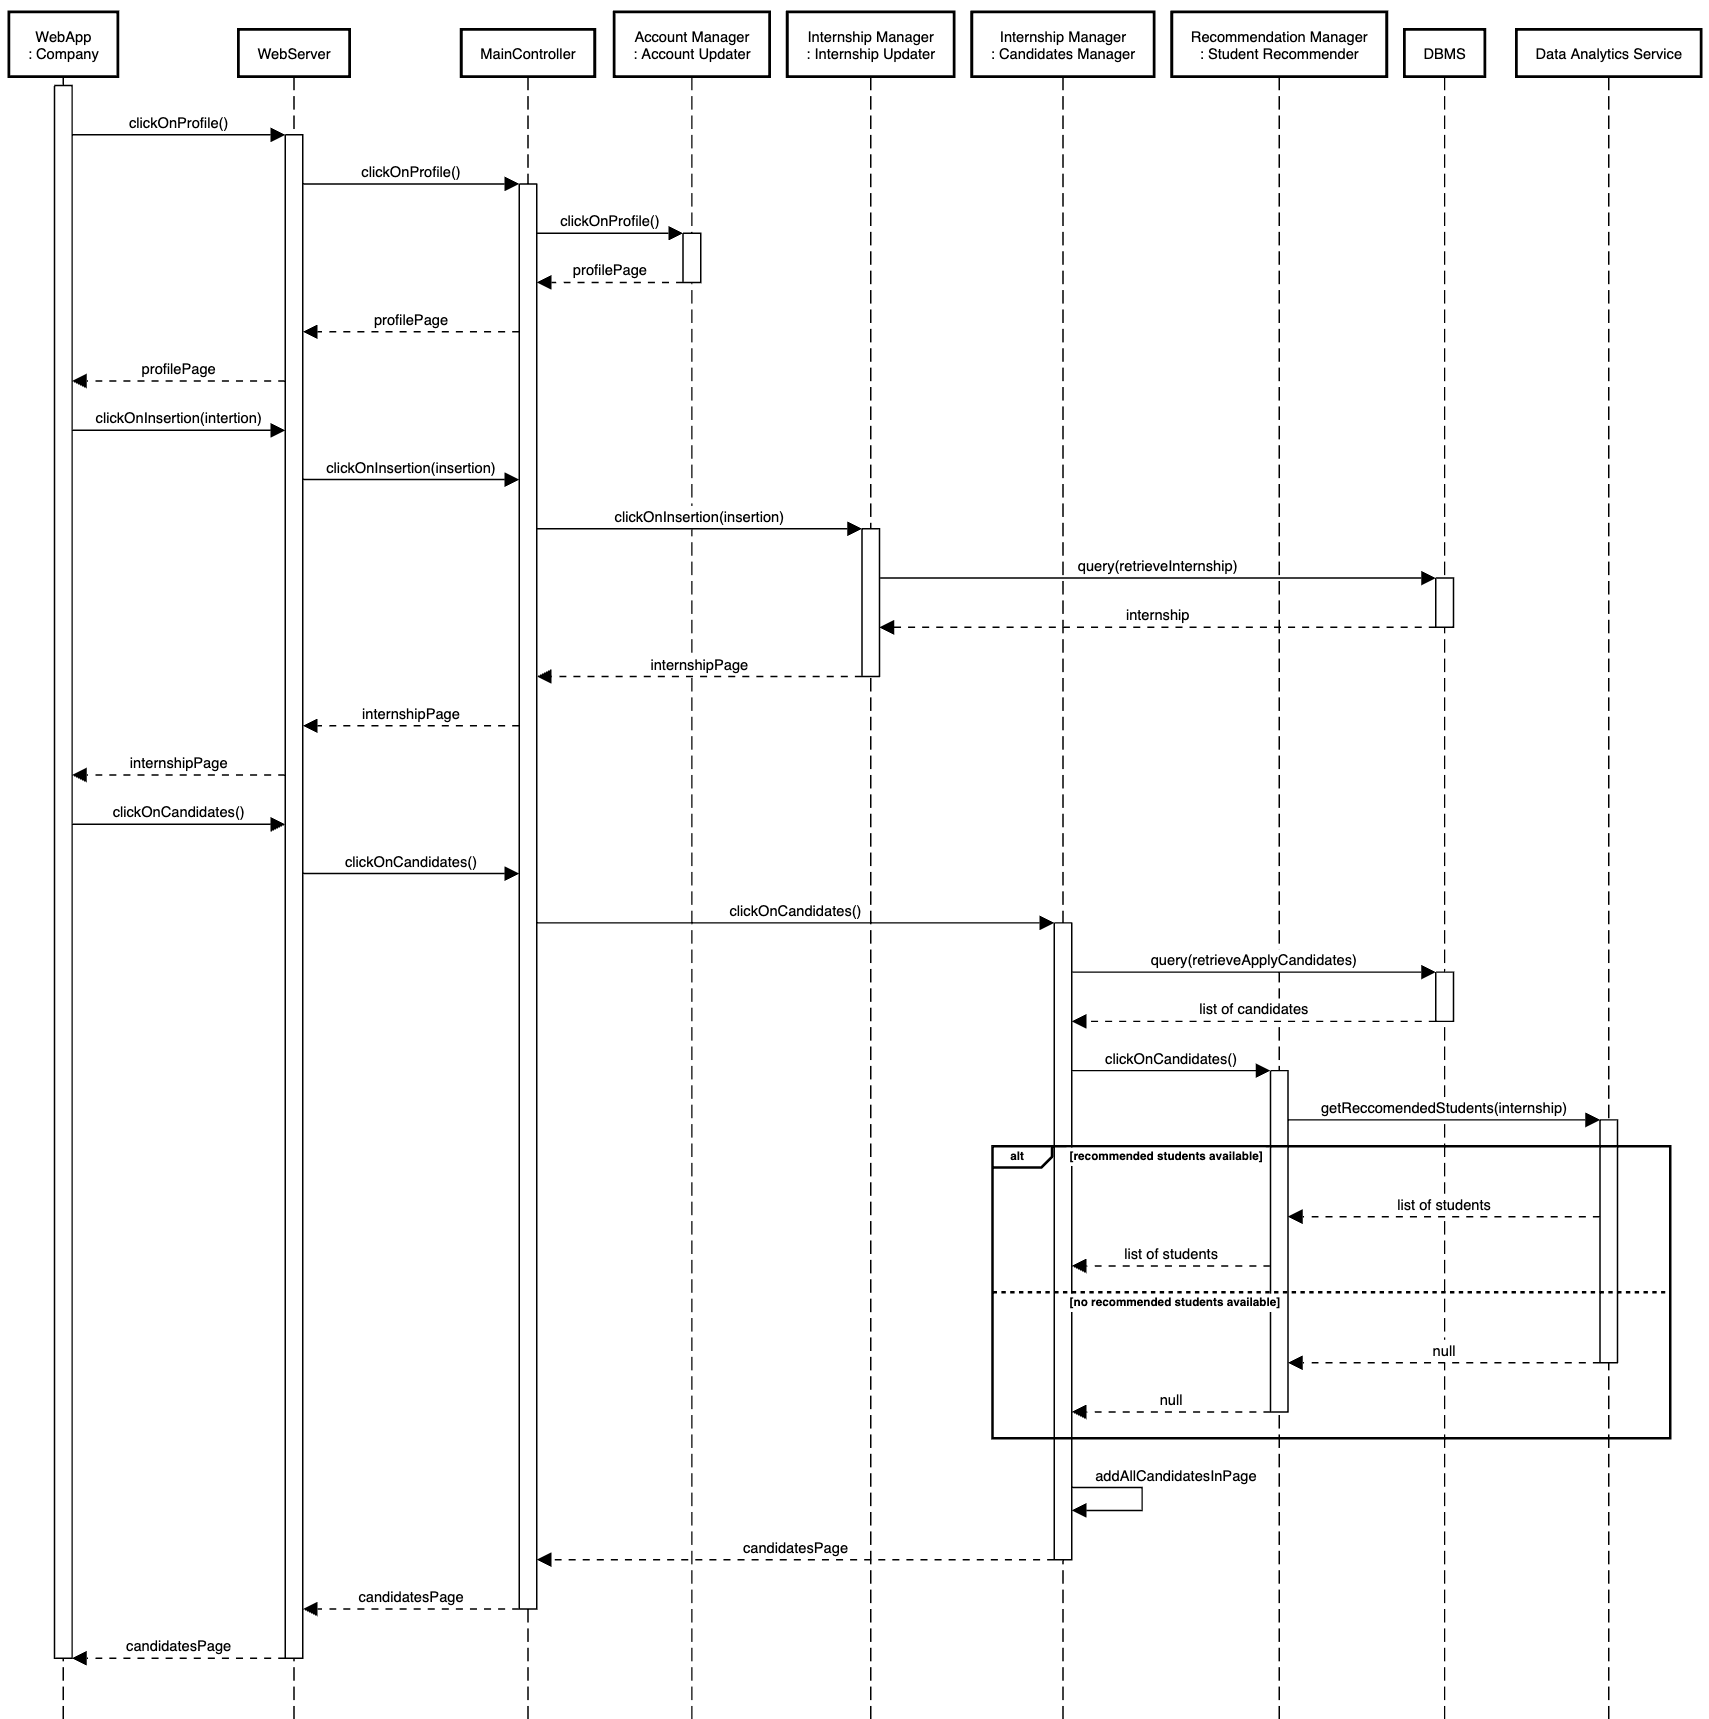
\includegraphics[width=\linewidth]{DD/Images/sequenceDiagrams/LookForRecommendedStudents.png}
    \caption{[UC11] Look for a student through recommended ones.}
    \label{fig:lookFrRecStudent_immagine}
\end{figure*}
\clearpage


The sequence diagram illustrates the process of a company looking for students through recommended profiles in the application. The company begins by clicking on their profile in the WebApp, which retrieves and displays the profile page via the WebServer and MainController. The company then selects an internship insertion they are offering, and the system retrieves and displays the internship details.

Next, the company clicks on the "candidates" option for the selected internship. The system retrieves the list of students who have applied for the internship from the database through the Candidates Manager. Simultaneously, the Recommendation Manager queries the Data Analytics Service for recommended students based on the internship details. If recommended students are available, their profiles are returned and added to the candidates page. If no recommended students are found, the system proceeds with only the applied candidates.

The candidates page is divided into two sections: one section lists the students who have applied for the internship, and the other section displays the recommended students whose profiles match the internship requirements. This layout allows the company to review both groups of students conveniently. The completed candidates page is then displayed to the company, concluding the process.

\begin{figure*}[htbp]
    \centering
    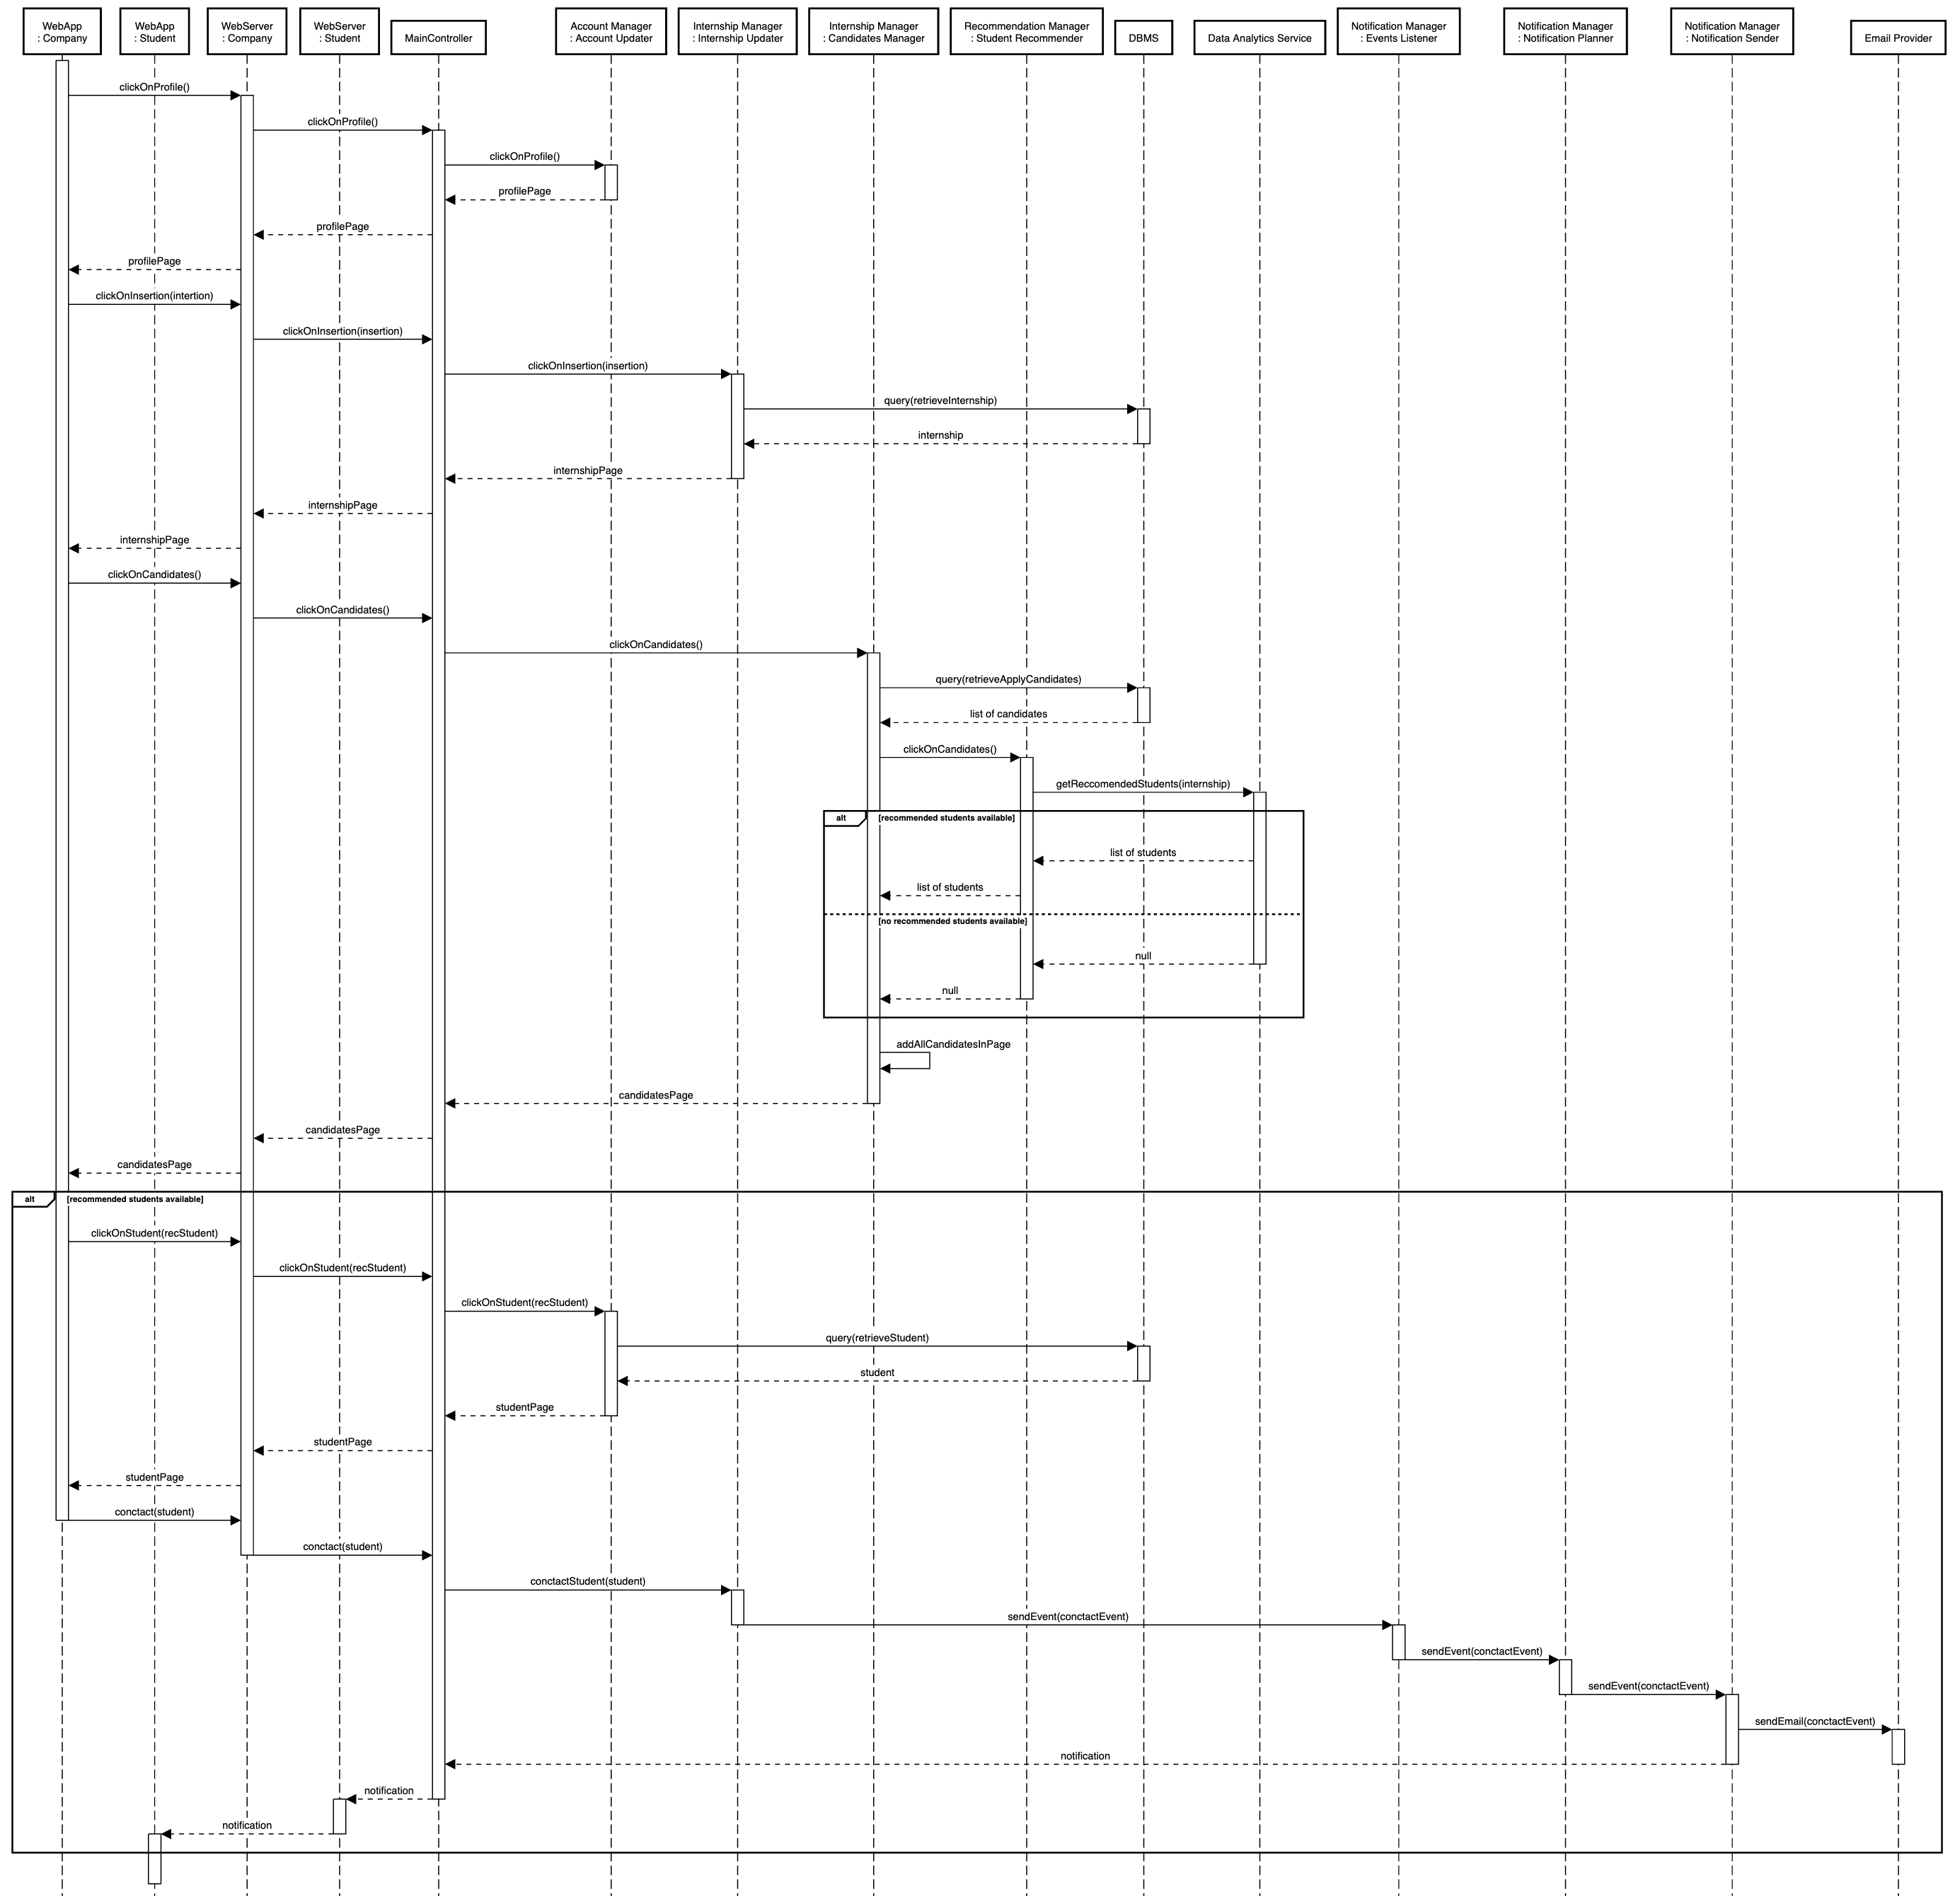
\includegraphics[width=\linewidth]{DD/Images/sequenceDiagrams/ContactRecStudent.png}
    \caption{[UC12] Contact a Recommended Student.}
    \label{fig:conctactRecStudent_immagine}
\end{figure*}
\clearpage

The sequence diagram illustrates the process of a company contacting a recommended student through the S\&C application. The company begins by clicking on their profile in the WebApp, which retrieves and displays the profile page via the WebServer and MainController. The company then selects an internship insertion they are offering, and the system retrieves and displays the internship details.

Next, the company clicks on the "candidates" option for the selected internship. The system retrieves the list of applied candidates from the database and queries the Data Analytics Service for recommended students through the Recommendation Manager. If recommended students are available, their profiles are added to the candidates page, which is divided into two sections: one for applied students and one for recommended students.

The company selects a recommended student, and the system retrieves the student's profile from the database. The profile is displayed to the company, who then initiates contact with the student. The MainController processes the contact request, triggering the Internship Updater to send a contact event to the Notification Manager. Notifications are sent via the Notification Planner and Notification Sender, and an email is sent to the student to inform them of the contact request. The WebApp also notifies the student, completing the process.

\newpage

\begin{figure*}[htbp]
    \centering
    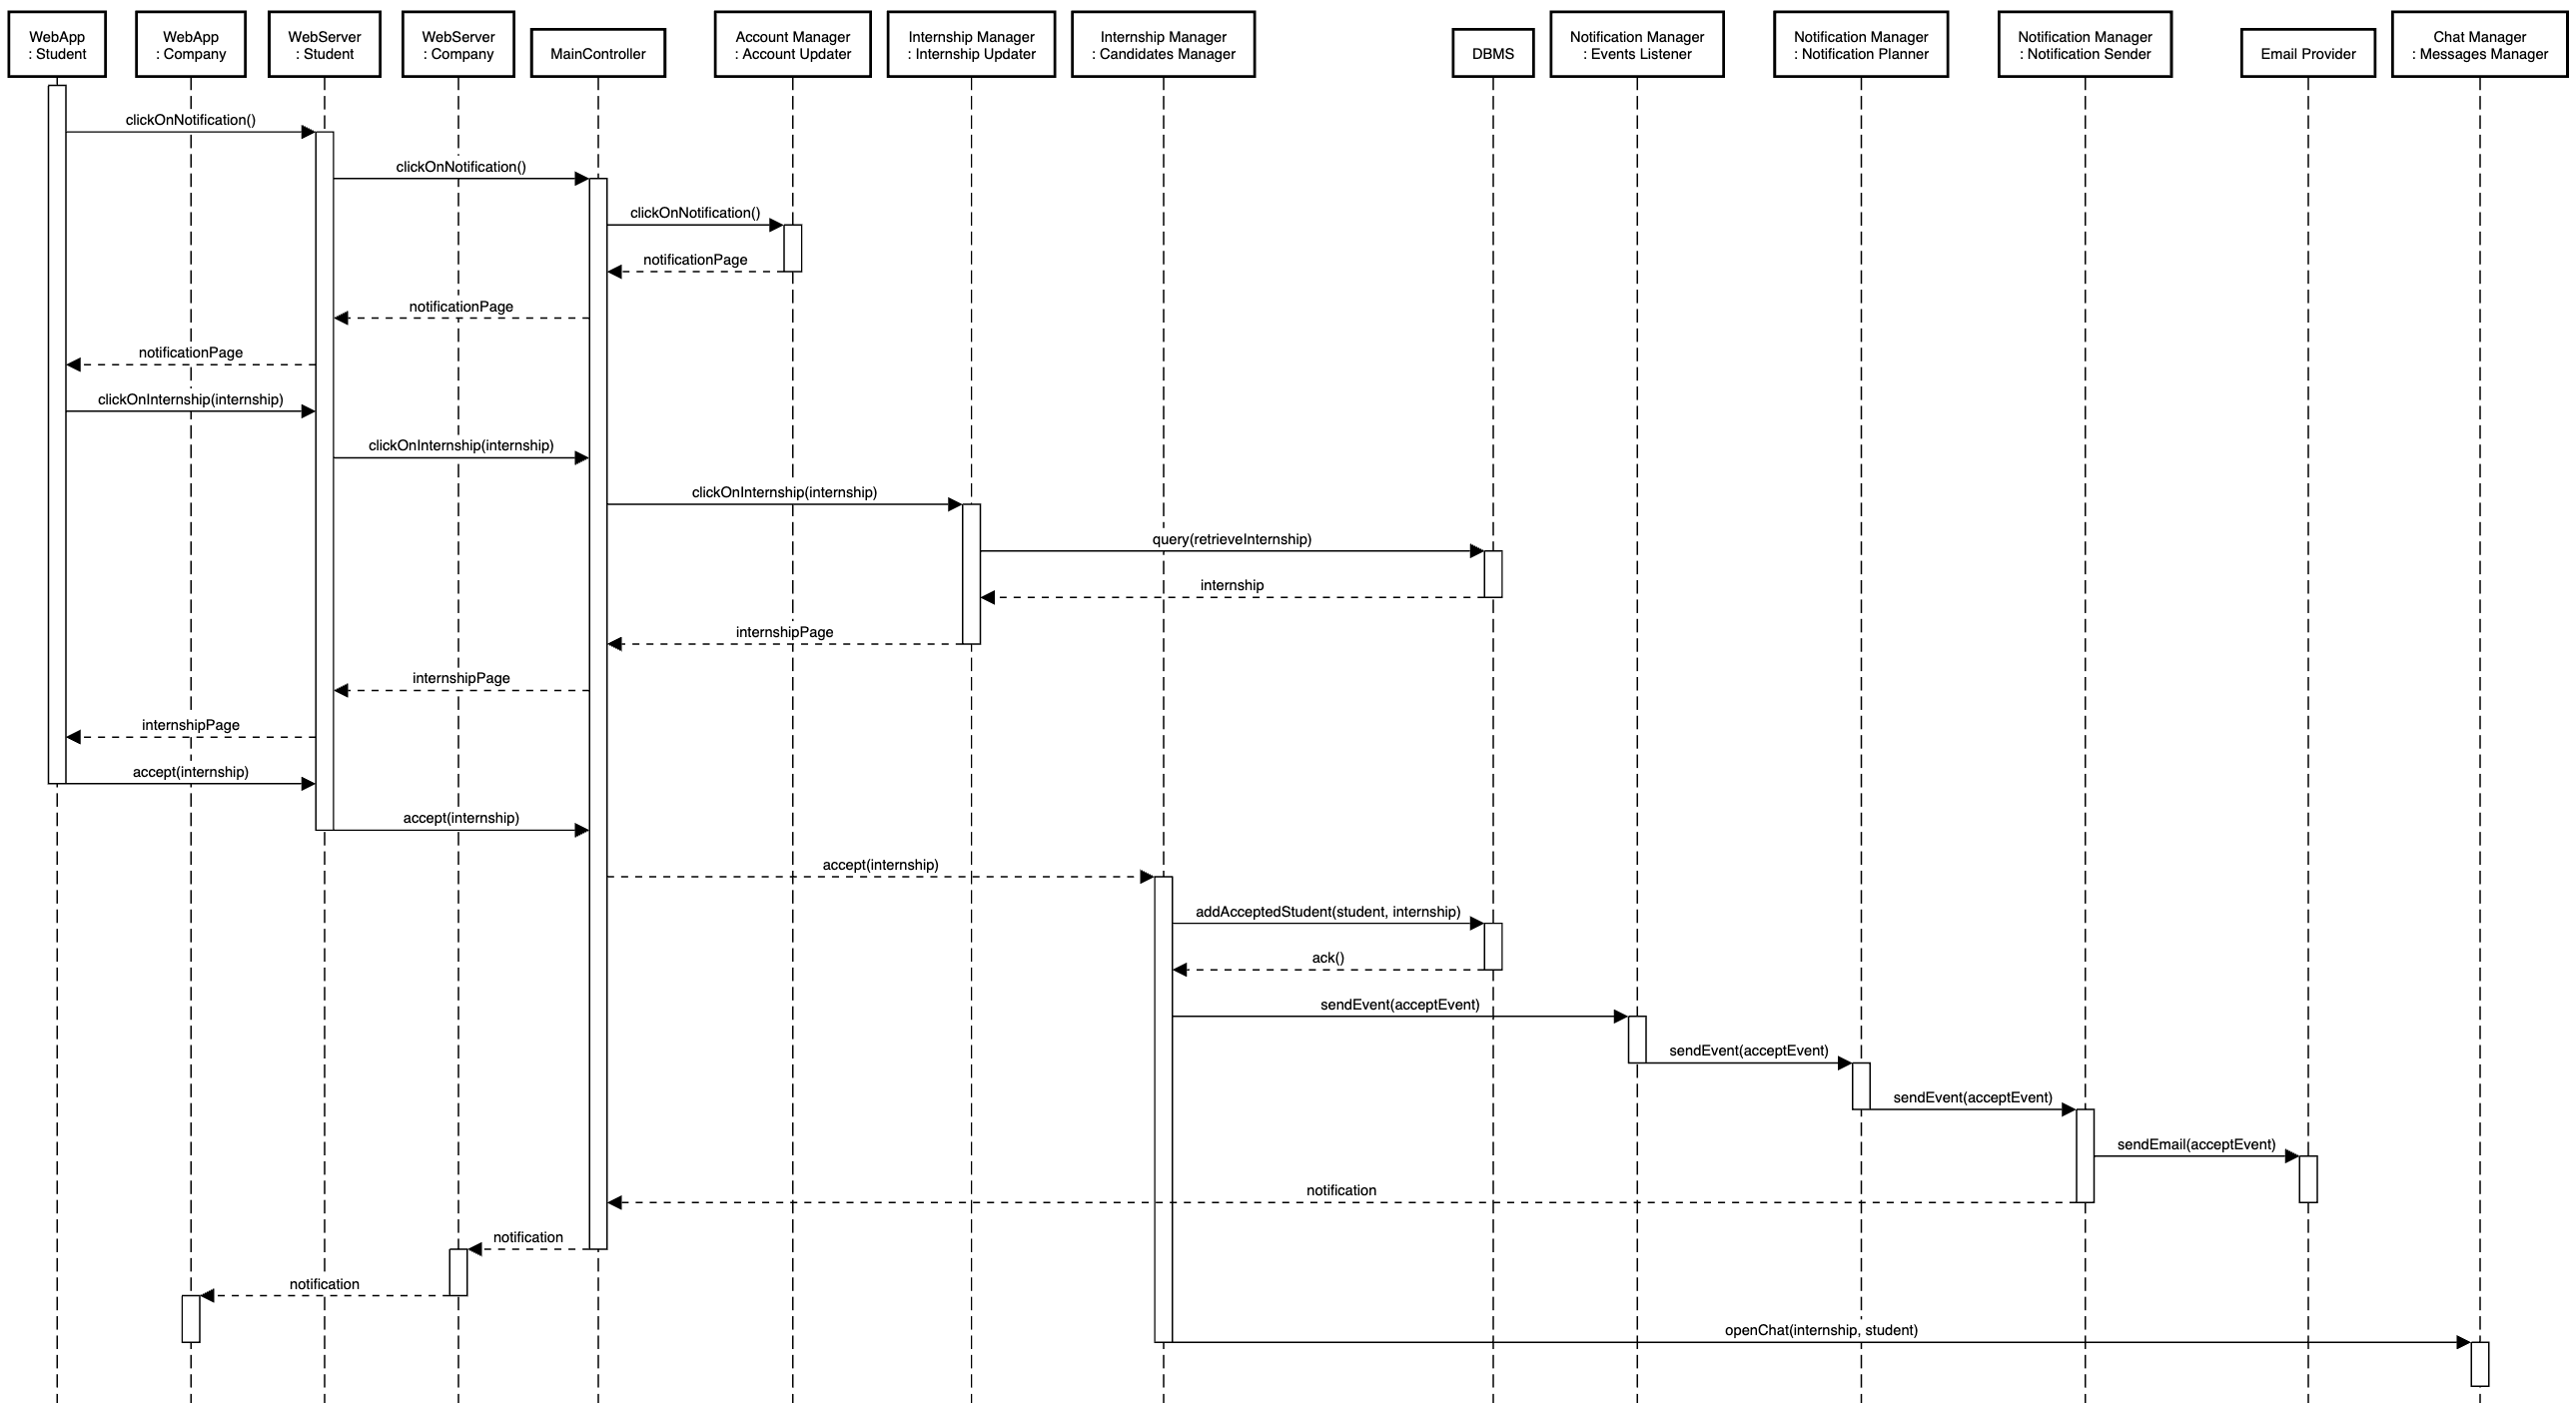
\includegraphics[width=\linewidth]{DD/Images/sequenceDiagrams/acceptCompany.png}
    \caption{[UC13] Accept a Company.}
    \label{fig:acceptCompany_immagine}
\end{figure*}



The sequence diagram illustrates the process of a student accepting a company for an internship through the S\&C application. The student starts by clicking on a notification in the WebApp, which retrieves and displays the notification page via the WebServer and MainController. The student selects the relevant internship from the notification page, and the system retrieves and displays the internship details.

The student then clicks "accept" for the internship. The WebServer sends the request to the MainController, which processes it through the Candidates Manager. The Candidates Manager updates the database to mark the student as accepted for the internship and triggers an event through the Notification Manager. Notifications are sent via the Notification Planner and Notification Sender, and an email is sent to the company to inform them of the student's acceptance. Additionally, a chat is opened between the student and the company for further communication, completing the process. 

\begin{figure*}[htbp]
    \centering
    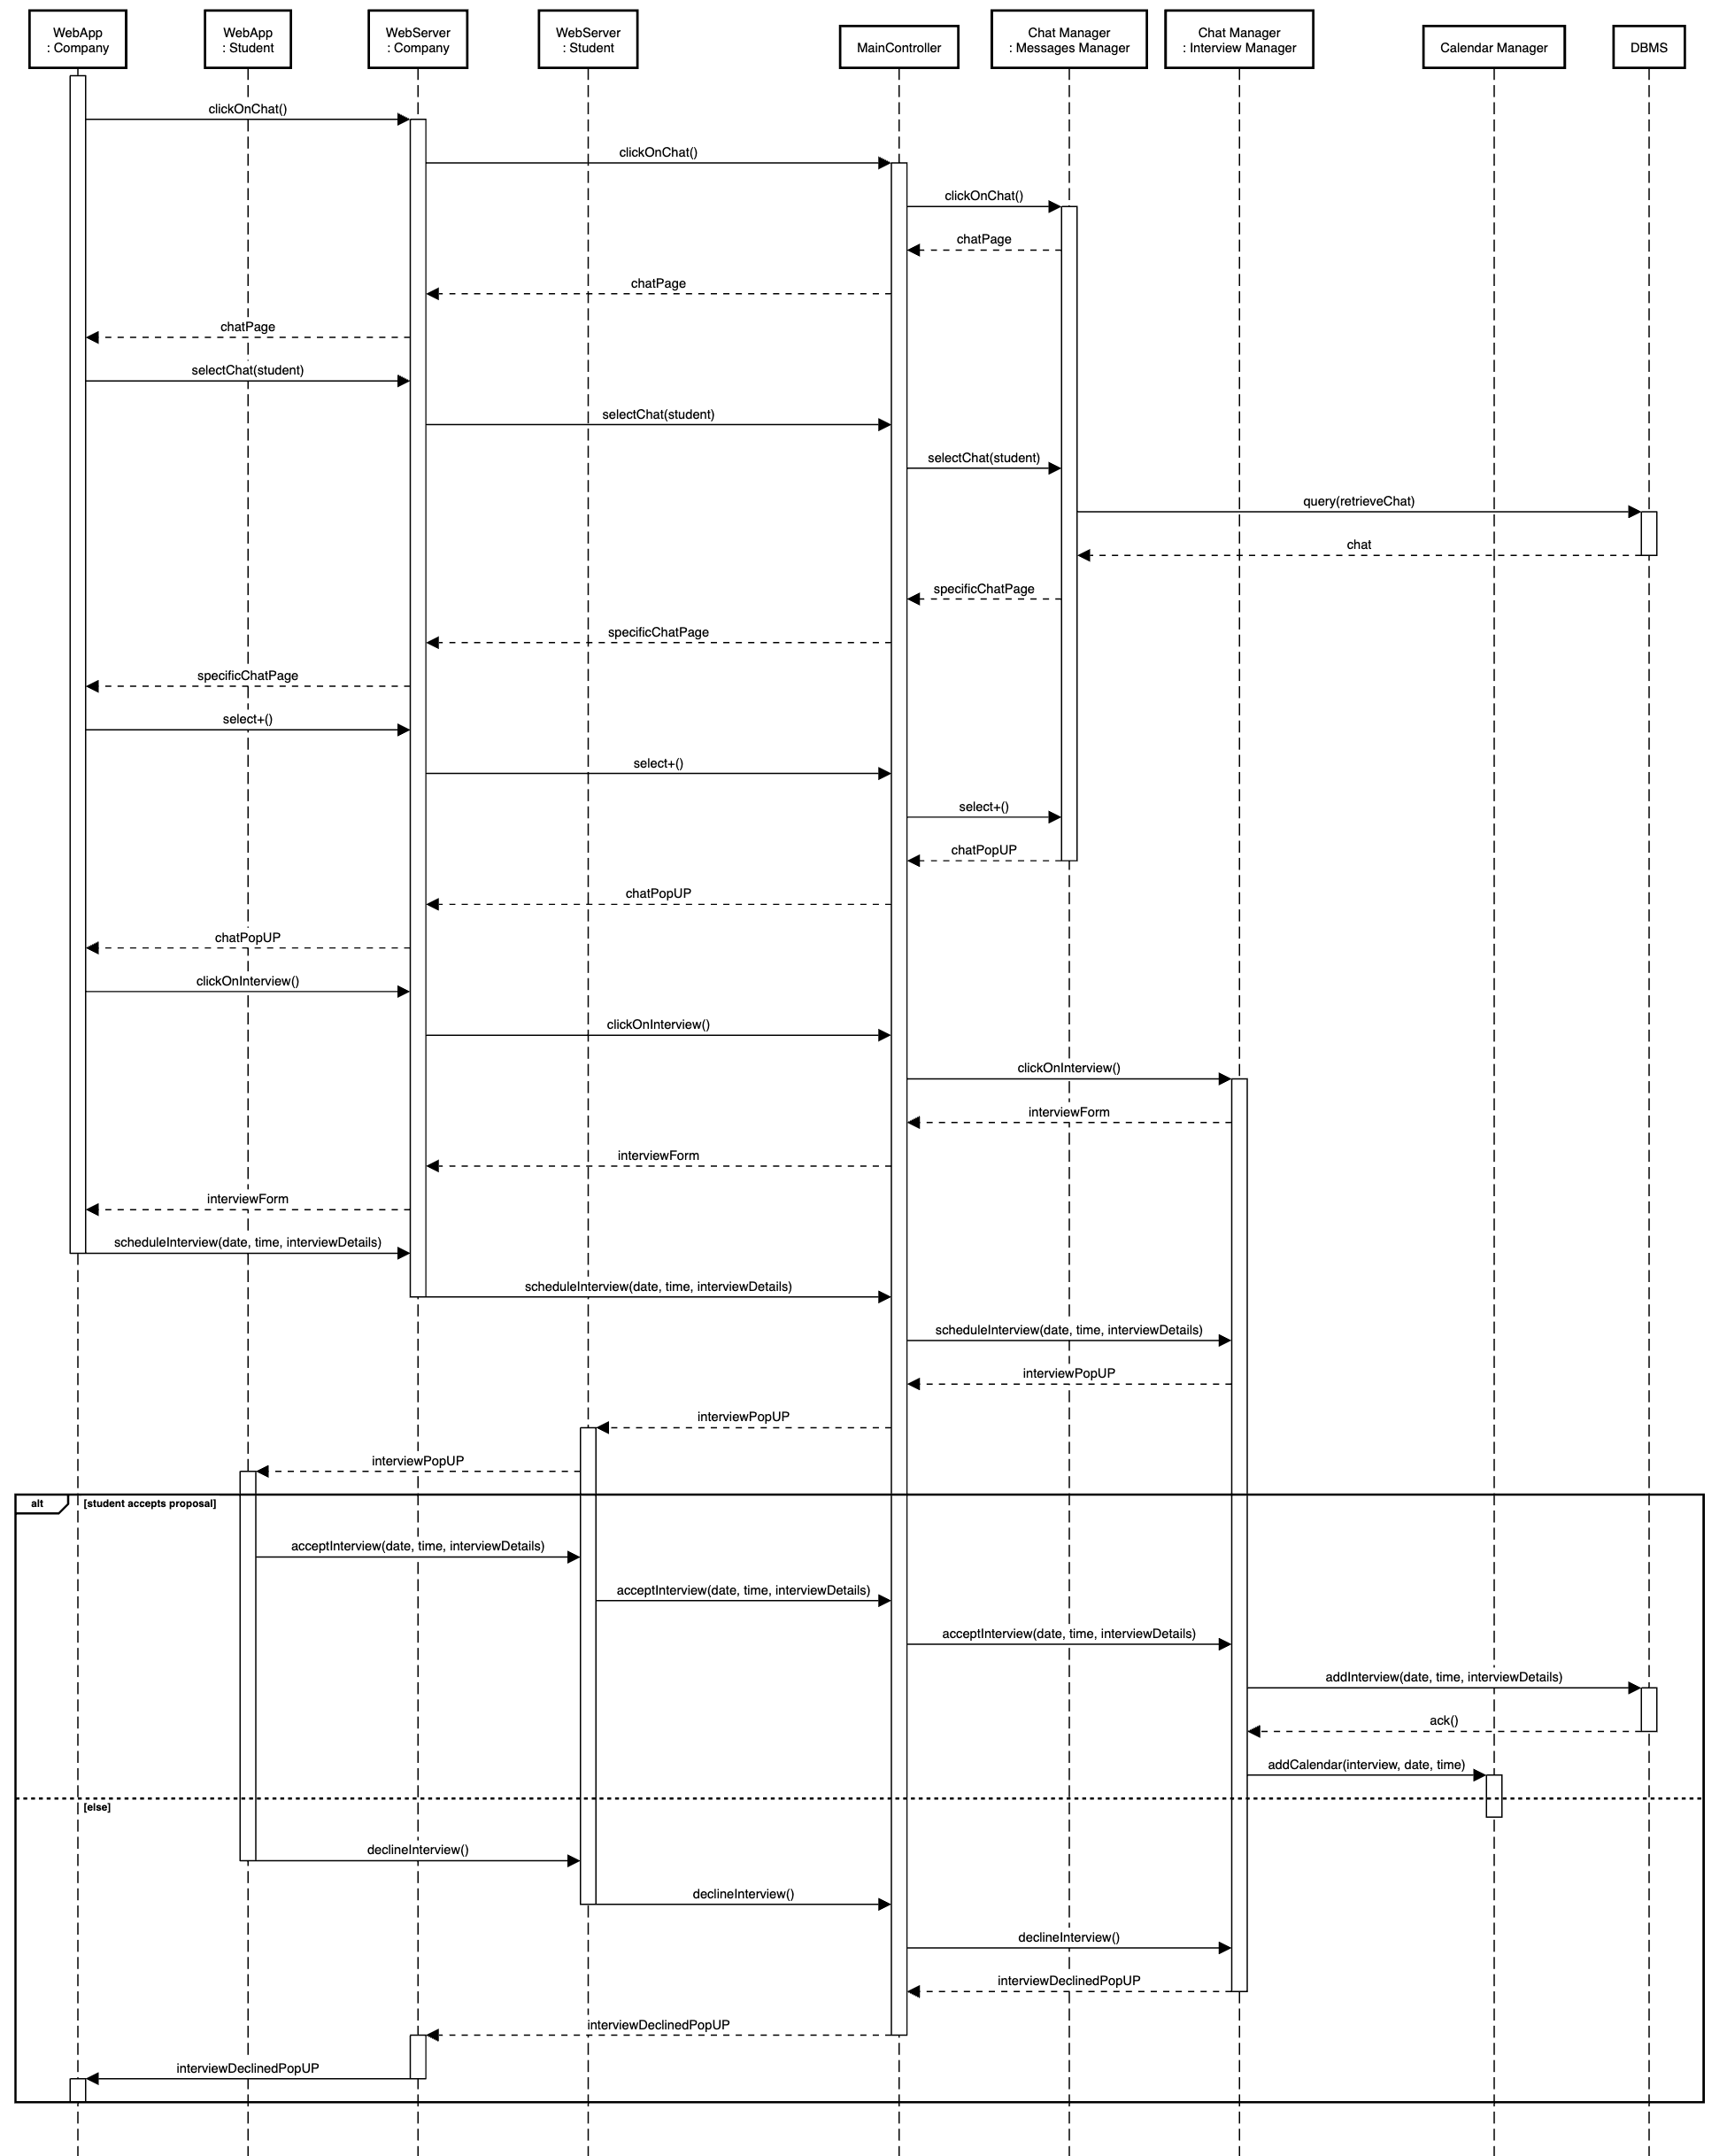
\includegraphics[width=\linewidth]{DD/Images/sequenceDiagrams/scheduleInterview.png}
    \caption{[UC14] Schedule an Interview.}
    \label{fig:scheduleInterview_immagine}
\end{figure*}
\clearpage


a student through the S\&C application. The company begins by clicking on the chat logo in the WebApp, which opens the chat page. The WebServer retrieves and displays the chat page. The company selects a specific chat with a student, and the system retrieves and displays the chat details.

Next, the company clicks on the "+" logo to open a popup with options and selects "interview." The system presents an interview scheduling form, where the company specifies the date, time, and details of the interview. The scheduling request is processed by the MainController and the Interview Manager, which prepares a notification for the student.

The student receives a popup notification about the interview proposal. If the student accepts the proposal, the Interview Manager adds the interview details to the database and updates the calendar through the Calendar Manager, adding the event. If the student declines, the system informs the company with a "declined interview" notification, completing the process.

\begin{figure*}[htbp]
    \centering
    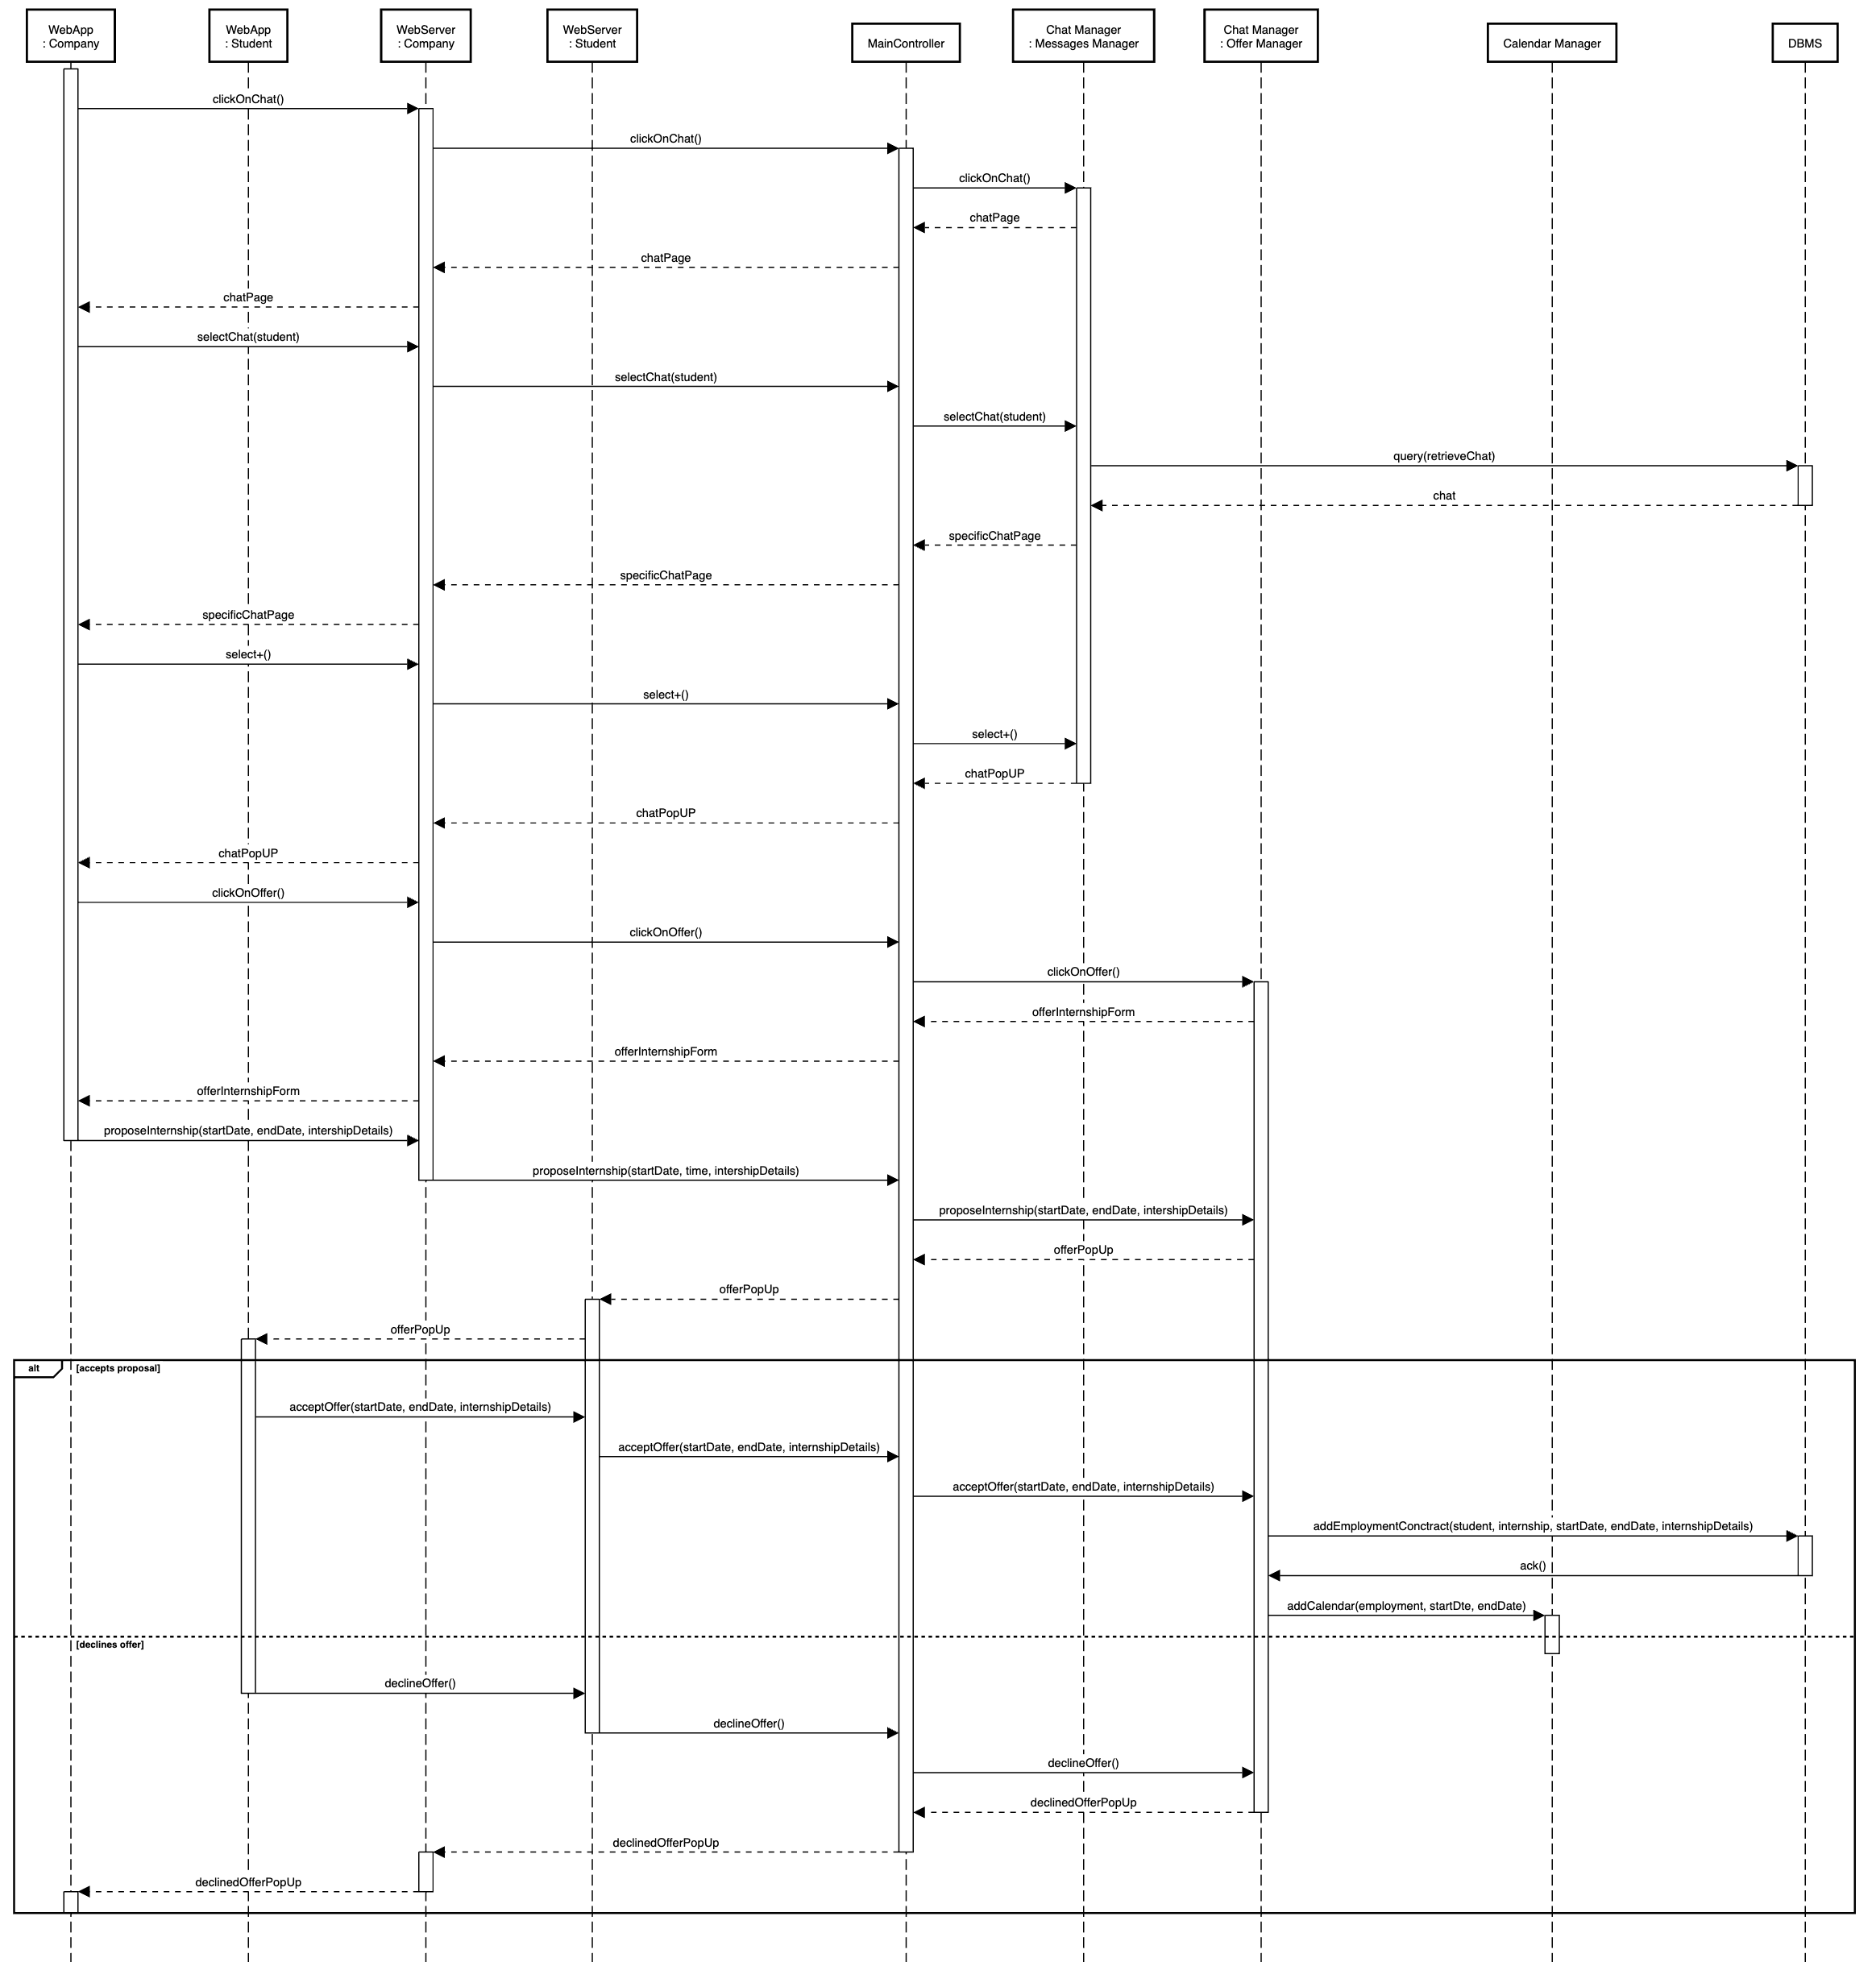
\includegraphics[width=\linewidth]{DD/Images/sequenceDiagrams/startInternship.png}
    \caption{[UC15] Start an Internship.}
    \label{fig:startInternship_immagine}
\end{figure*}
\clearpage


The sequence diagram illustrates the process of a company proposing an internship offer to a student through the S\&C application. The company starts by clicking on the chat logo in the WebApp, which opens the chat page. The WebServer retrieves and displays the chat page. The company selects a specific chat with a student, and the system retrieves and displays the chat details.

Next, the company clicks on the "+" logo to open a popup with options and selects "offer." The system presents an internship offer form, where the company specifies the start date, end date, and other internship details such as the workplace, remuneration, tasks, and other relevant information. Once the company submits the offer, the MainController processes the request through the Offer Manager, which sends a notification to the student.

The student receives a popup notification about the internship offer. If the student accepts, the Offer Manager updates the database by adding an employment contract with the provided details and updates the calendar with the internship dates. The event is added to both the student’s and the company’s calendars. If the student declines the offer, the system notifies the company with a "declined offer" popup, completing the process.

\begin{figure*}[htbp]
    \centering
    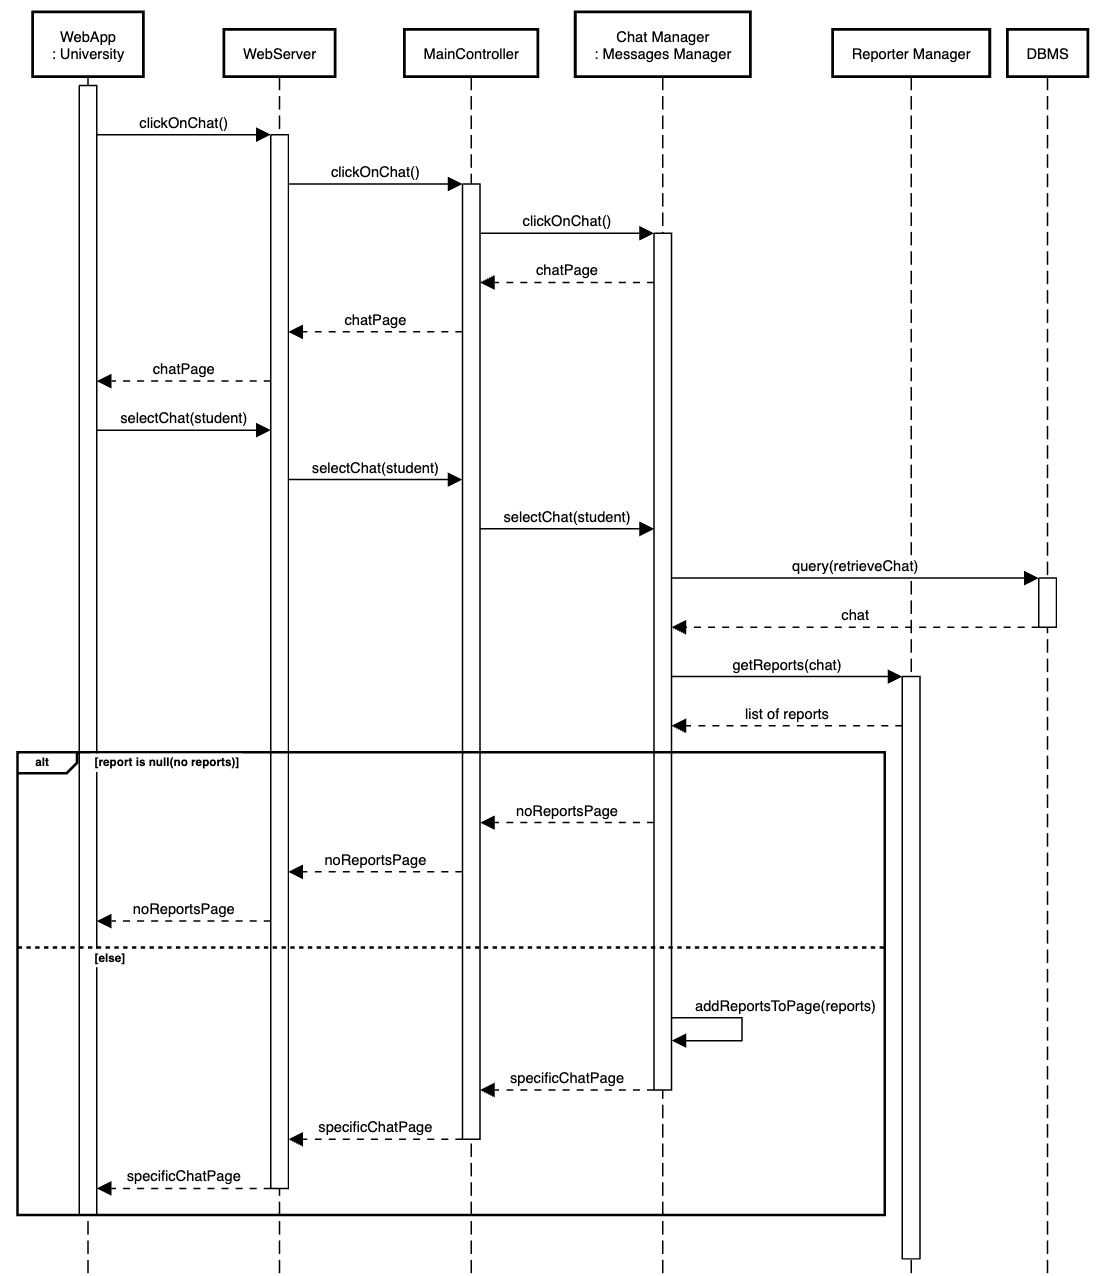
\includegraphics[width=\linewidth]{DD/Images/sequenceDiagrams/monitorInternship.png}
    \caption{[UC16] Monitor internship.}
    \label{fig:monitorInternship_immagine}
\end{figure*}
\clearpage



The Sequence diagram illustrates the process of a university monitoring the internship of one of its enrolled students through the S\&C application. The university begins by clicking on the chat logo in the WebApp, which opens the chat page. The WebServer retrieves and displays the chat page.

The university selects a specific chat with a student, and the system retrieves the chat details from the database. Additionally, the system queries the Reporter Manager to fetch any associated reports (information or complaints) related to the selected chat.

If no reports are available, the system displays a "no reports" page to the university. If reports are found, they are added to the chat page, and the updated chat page with the reports is displayed. This ensures that the university can monitor both the interactions and any reports submitted by the student or the company. This process keeps the university informed about the internship's status and any potential issues requiring intervention.

\newpage

\begin{figure*}[htbp]
    \centering
    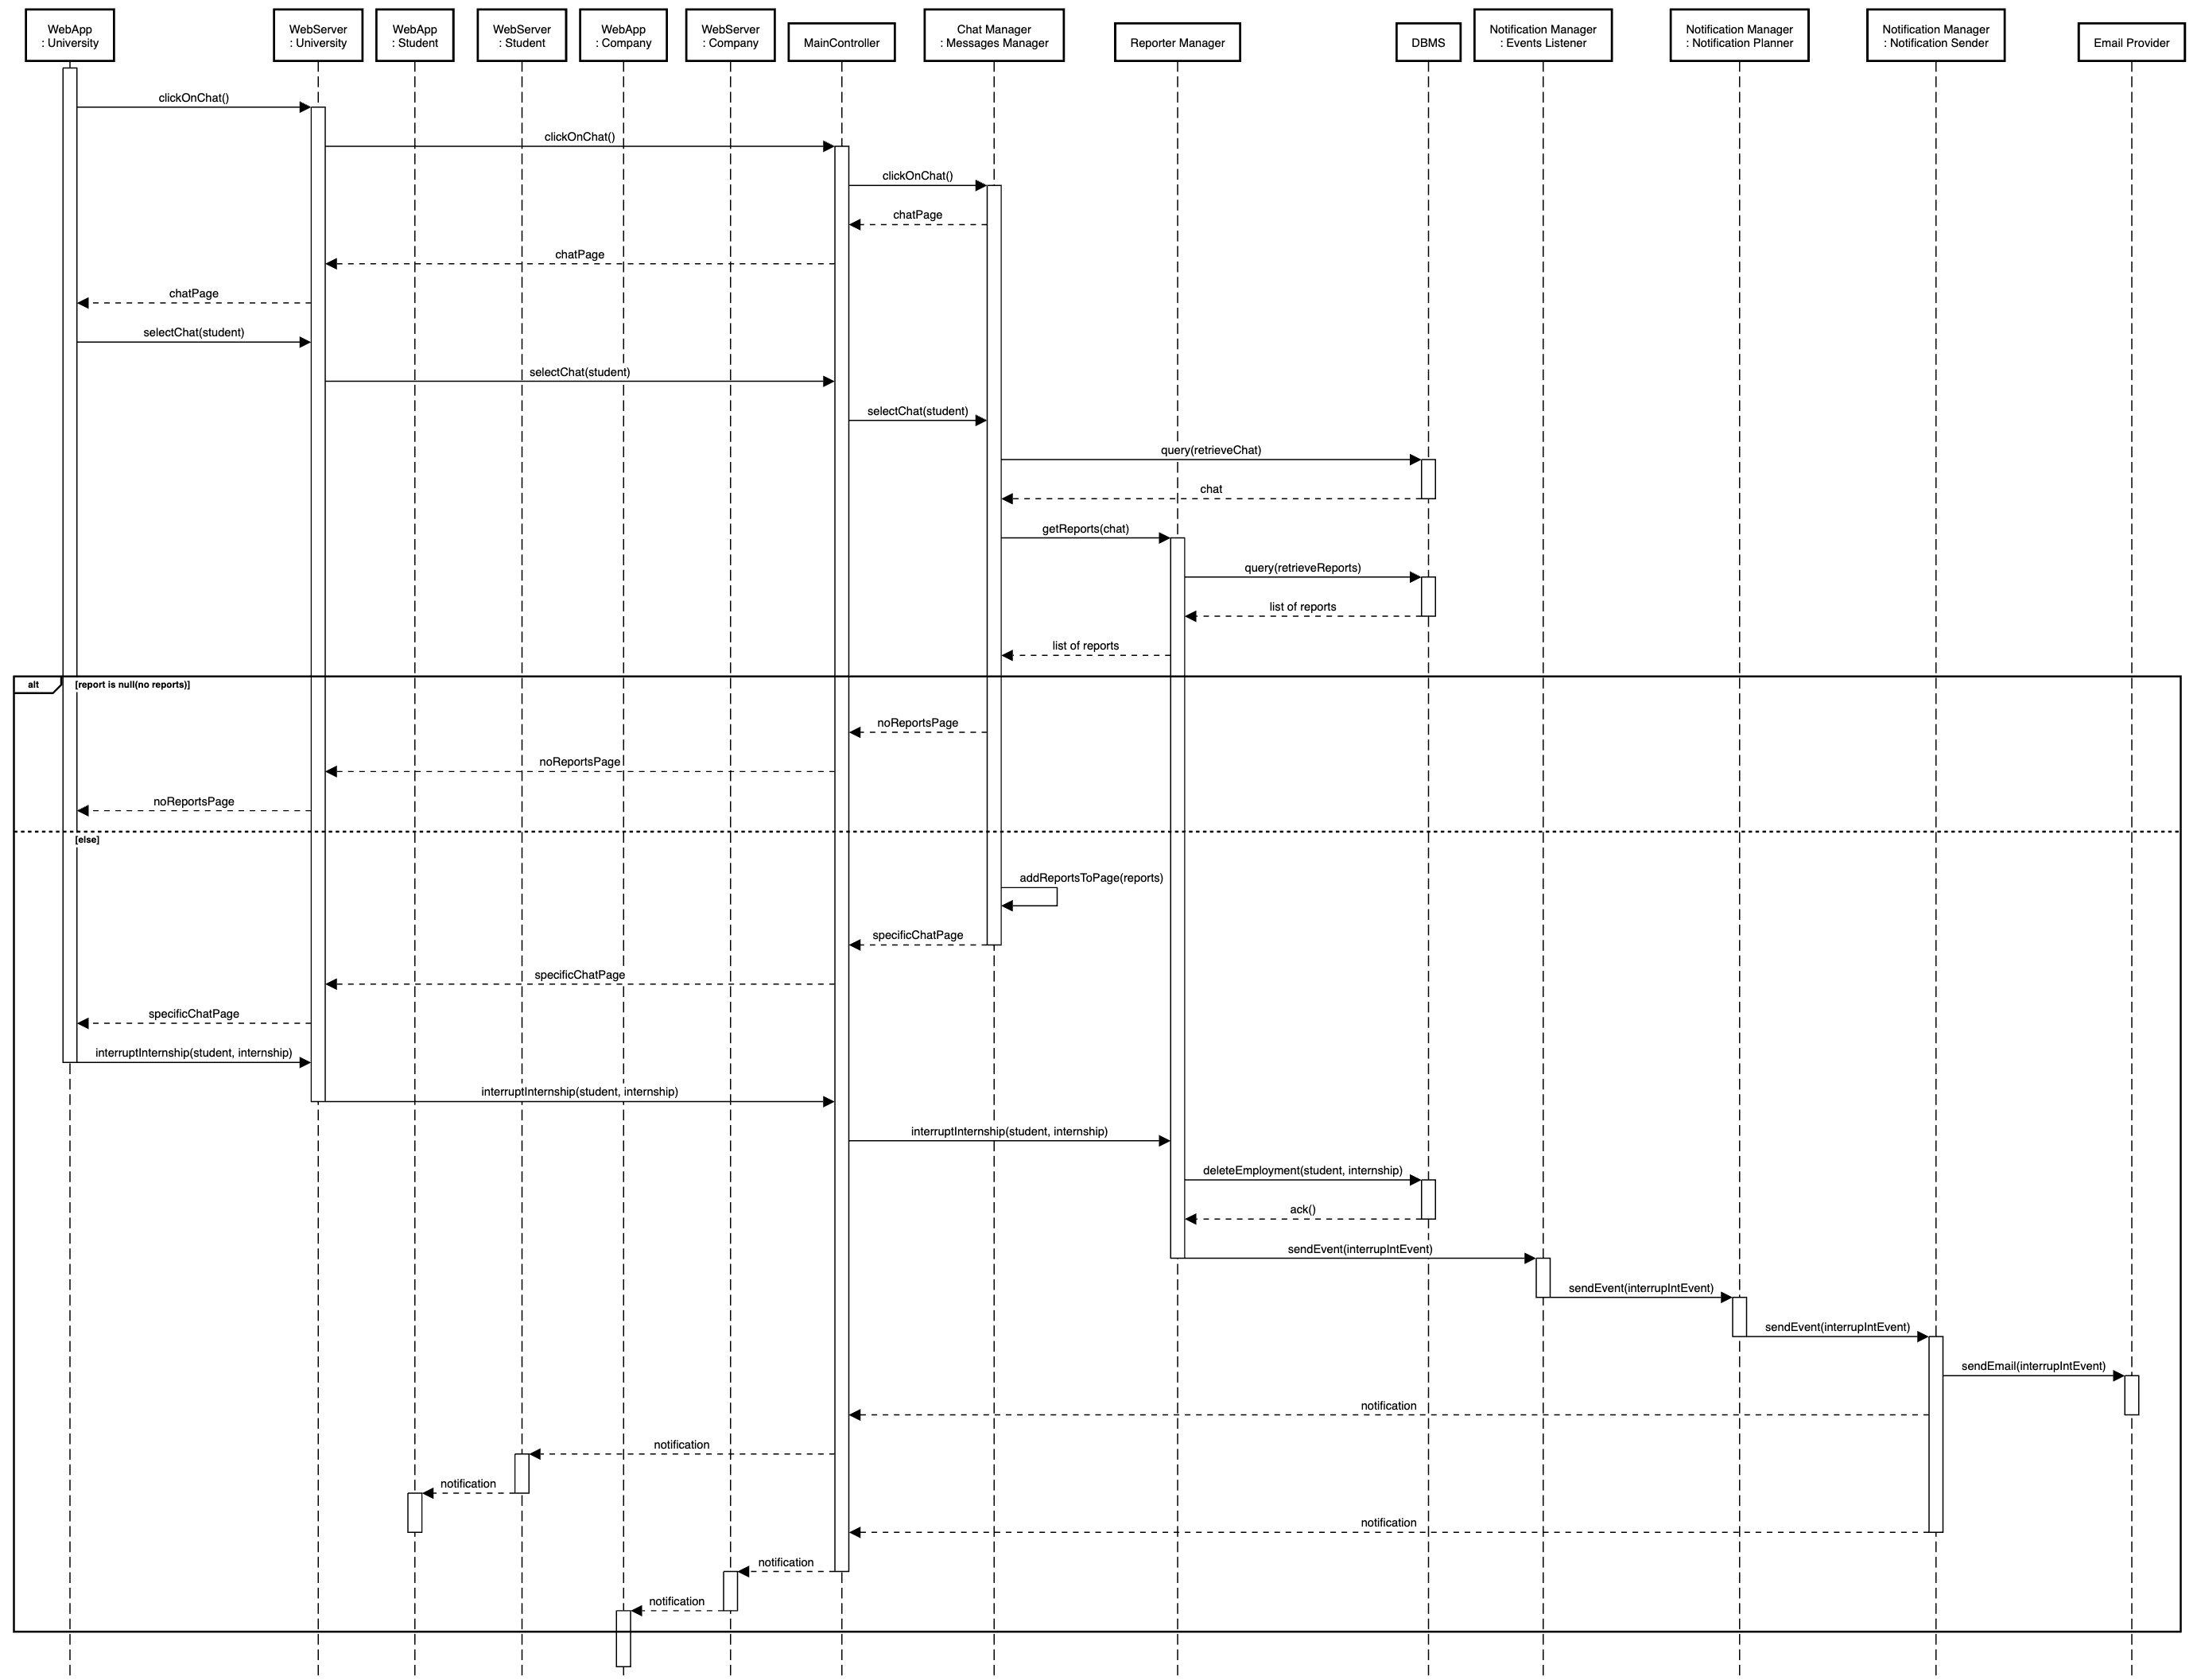
\includegraphics[width=\linewidth]{DD/Images/sequenceDiagrams/interruptInternship.png}
    \caption{[UC17] Interrupt internship.}
    \label{fig:interruptInternship_immagine}
\end{figure*}



The sequence diagram illustrates the process of a university interrupting a student's internship through the S\&C application when complaints are present and deemed necessary. The university begins by clicking on the chat logo in the WebApp, which opens the chat page. The WebServer retrieves and displays the chat page.

The university selects a specific chat with a student, and the system retrieves the chat details from the database. It also queries the Reporter Manager to fetch any associated reports (information or complaints) related to the internship. If no reports are found, the system displays a "no reports" page. If reports are available, they are added to the chat page, and the updated page is displayed to the university.

If the university determines that the complaints warrant intervention, it selects the "interrupt internship" option. The WebServer sends the request to the MainController, which forwards it to the Reporter Manager. The Reporter Manager deletes the employment record from the database, effectively terminating the internship.

The Reporter Manager then triggers an event through the Notification Manager. Notifications are processed and sent via the Notification Planner and Notification Sender. An email is sent to all relevant parties, and notifications are displayed to both the student and the company through their respective WebApps, informing them of the internship's termination. This ensures that all stakeholders are promptly informed of the decision.









\newpage

\section{Selected Architectural Styles and Patterns}
\label{sec:sel_arch_styles_patterns}%

The architectural design of the S\&C system leverages a 4-tier architecture, combining well-established architectural styles and design patterns to ensure scalability, maintainability, and ease of integration.

The system separates concerns across distinct layers:

\begin{itemize}
    \item 
        \textbf{Presentation Layer:} Provides the user interface through a web application. This layer focuses on user interaction and performs basic checks, such as form validation, delegating all business logic to the application server.
    \item 
        \textbf{Web Layer:} Acts as an intermediary, forwarding requests between the presentation layer and the application server while ensuring secure communication.
    \item 
        \textbf{Application Layer:} Implements all the business logic of the system. This layer consists of modular components, each responsible for specific functionalities.
    \item 
        \textbf{Data Layer:} Manages the storage and retrieval of data, ensuring consistency and persistence.
\end{itemize}

The separation of these layers ensures that the system is modular and can be scaled or modified without significant changes to other tiers. The separation between the Web Server and the Application Server was primarily motivated by the enhanced security this approach typically provides. Additionally, this decision positively impacts the system's development process by enabling parallel work across different tiers, allowing multiple teams to collaborate efficiently and expedite implementation.

\subsection{Model-View-Controller (MVC)}
\label{subsec:mvc}%

The \textbf{MVC pattern} is applied to the presentation and application server layers, enabling a clear separation between the user interface (View), user interactions (Controller), and business logic (Model). This structure simplifies the management of the web application’s user interface, allowing the frontend and backend to be developed independently. By isolating business logic from the presentation layer, the pattern ensures that updates to the user interface can be made without impacting the underlying logic, promoting maintainability and scalability.

\subsection{Centralized Access}
\label{subsec:centralized_access}%

The Main Controller simplifies interactions by acting as a \textbf{facade} between the Web Server and backend components. This centralization reduces complexity, ensuring that the Web Server interacts with a unified interface rather than managing connections to multiple components. By consolidating these interactions, the system achieves greater modularity and ease of maintenance. Additionally, the Main Controller enables the implementation of shared logic, such as authentication, validation and error handling, in a single location. This approach avoids duplication across components and ensures consistency in enforcing security policies and logging activities. 

This design also enhances scalability and debugging. With all requests passing through the Main Controller, load management can be centralized, and system behavior can be easily monitored. This approach reduces coupling between tiers, supporting the system's ability to adapt to future changes or expansions.

\subsection{Observer Pattern}
\label{subsec:observer_pattern}%

The \textbf{Notification Manager} leverages this pattern by subscribing to specific events, such as registration completion or new internship postings, and triggering notifications in response. By decoupling event handling from the core logic of other components, this approach ensures that components remain loosely coupled, reducing dependencies on the notification system. This design enhances modularity and extensibility, allowing new event types or notification methods to be added without impacting the rest of the system.

\subsection{Repository Pattern}
\label{subsec:repository_pattern}%

The \textbf{repository pattern} is used to abstract database operations, enabling the application server to interact with data through well-defined, high-level interfaces. This abstraction ensures consistency in how data is accessed and manipulated, while also reducing redundancy in database queries. By centralizing database interactions, this pattern improves maintainability, providing a single source of truth and making it easier to adapt to changes in the underlying data structures or queries.

\newpage

\section{Other design decisions}
\label{sec:other_design_dec}%

Beyond the core architectural styles and patterns, several additional design decisions were made to address specific challenges and enhance system functionality:

\subsection{Event-Driven Asynchronous Processing}

To maintain responsiveness and scalability, \textbf{asynchronous processing} was adopted for tasks like sending notifications. This ensures that user interactions remain smooth and uninterrupted, while heavy operations are handled independently.

\subsection{Security Enhancements}

The system enforces \textbf{HTTPS} for all communication between tiers to safeguard data in transit. Additionally, encryption is applied to sensitive data stored in the database, and Role-Based Access Control (RBAC) restricts user permissions based on their roles (e.g., student, company, or administrator).

\subsection{Database Query Optimization}

Frequent \textbf{queries}, such as internship searches or user profile retrievals, were optimized through indexing and caching mechanisms. These optimizations ensure high performance, particularly as the system scales to accommodate more users.

\subsection{Integration Flexibility}

\textbf{External integrations}, such as AI tools for CV enhancement and analytics for recommendations, were designed to be \textbf{modular}. This allows new services to be incorporated with minimal changes to the system, supporting adaptability to future requirements.

\subsection{Error Logging and Monitoring}

A unified \textbf{error-handling} and \textbf{logging framework} was implemented across all tiers. This approach facilitates debugging and ensures system administrators can monitor performance and address issues promptly.
